\section{Results}\label{results}

\subsection{Code testing}

The IIEE module being implemented, some tests were required in order to check that the code behaves accordingly. To do so, several tests were realised. The first one consisted of statistical results for the yield. To derive a statistics, the simple geometry from \ref{Theory_axy} was implemented, as well as several horizontal slices of ions. These ions were initialised at different radial distances from the cathode. Making use of Eq.(\ref{ions_energy}), their energy as they hit the electrode is known, and so is the average yield per incident ion. Recall that the yield is a function of the incident ion energy only, through the energy loss in the material,

\beq
\gamma(E) = \Lambda_{exp}\cdot \frac{dE}{dx}\Bigg|_i.\label{yield_result}
\eeq 

\noindent It is also important to note that the energy loss tables used to implement the yield curves as in Fig.(\ref{yield}) contained values for protons impinging on different materials. In order to obtain results exploitable for the TREX experiment, the yield for incident protons had to be replaced by the yield for other ions, as H$_2^{+}$ for example. Approximatively, since H$_{2}$ is a diatomic molecule formed of hydrogen atoms, which are protons when ionised, one can deduce the yield for H$_2^{+}$ cations through $dE(\tilde{E})/dx|_{H_2^{+}} \sim 2dE(\tilde{E}/2)/dx|_{H^{+}}$ \cite{Yield_H2}. Hence, Eq.(\ref{yield_result}) reads 

\beq
\gamma_{H_2^+}(\tilde{E}) = \Lambda_{exp}\cdot \frac{dE(\tilde{E})}{dx}\Bigg|_{H_2^+} =2 \Lambda_{exp}\cdot \frac{dE(\tilde{E}/2)}{dx}\Bigg|_{H^+},
\eeq  

and then 

\beq
\gamma_{H_2^+}(E) \simeq 2\cdot \gamma_{H^+}(E/2). \label{Yield_H2+}
\eeq
\noindent For all three materials, the slices of ions were initialised along the axial direction, thus enabling to show that the electron generation from the code, over the loss of ions, is independent of the axial position, as expected. Fig.(\ref{flat_slice}) shows the results for $H_2^{+}$ cations impinging on the cathode made either of $^{304}$SS, Cu or Al. The potential bias applied between the two electrodes is $\Delta \phi=20$ kV. The magnetic field is uniform, with field lines parallel to the electrodes, and $B=0.21$ T, as it is a value of the order of magnitude used in gyrotrons. The radial positions of the electrode were $r_a=0.001$ m for the cathode and $r_b=0.01$ m for the anode, and the ions were generated at $r_1 = 0.003$ m, $r_2=0.005$ m and $r_3=0.008$ m. Using the very simple equation Eq.(\ref{Yield_H2+}), the expected yield could be estimated and the comparison of the latter with the one obtained from the IIEE module is exposed in Table.(\ref{tab_stat}). 

\begin{figure}[h!]
\centering
	\includegraphics[width = 1.0 \textwidth]{Flatslice_stats.eps}
	\caption{\label{flat_slice} Plot of the number of particles over the number of time-steps. The black curve represents the number of ions, while the colored curves show the number of electrons produced in the impingement of $H_2^+$ ions over $^{304}$SS, Cu and Al.}
\end{figure}  

\noindent One notes on Fig.(\ref{flat_slice}) that the ions population curve is discontinuous. It is due to the fact that the ions are initially configured in three slices at distinct radii, as shown in Fig.(\ref{slice_config}), and together with the symmetry of the system, they reach the cathode and disappear at distinct discrete times, hence the steps. Regarding the peaked shape of the electronic population curves, they disappear few time after being generated because in this geometry, the magnetic field lines are parallel to the electrodes. Thus, of a Larmor gyration, the electrons are not moving away from the cathode, and hence, they are recaptured few after being emitted.\\

\begin{figure}[h!]
\centering
	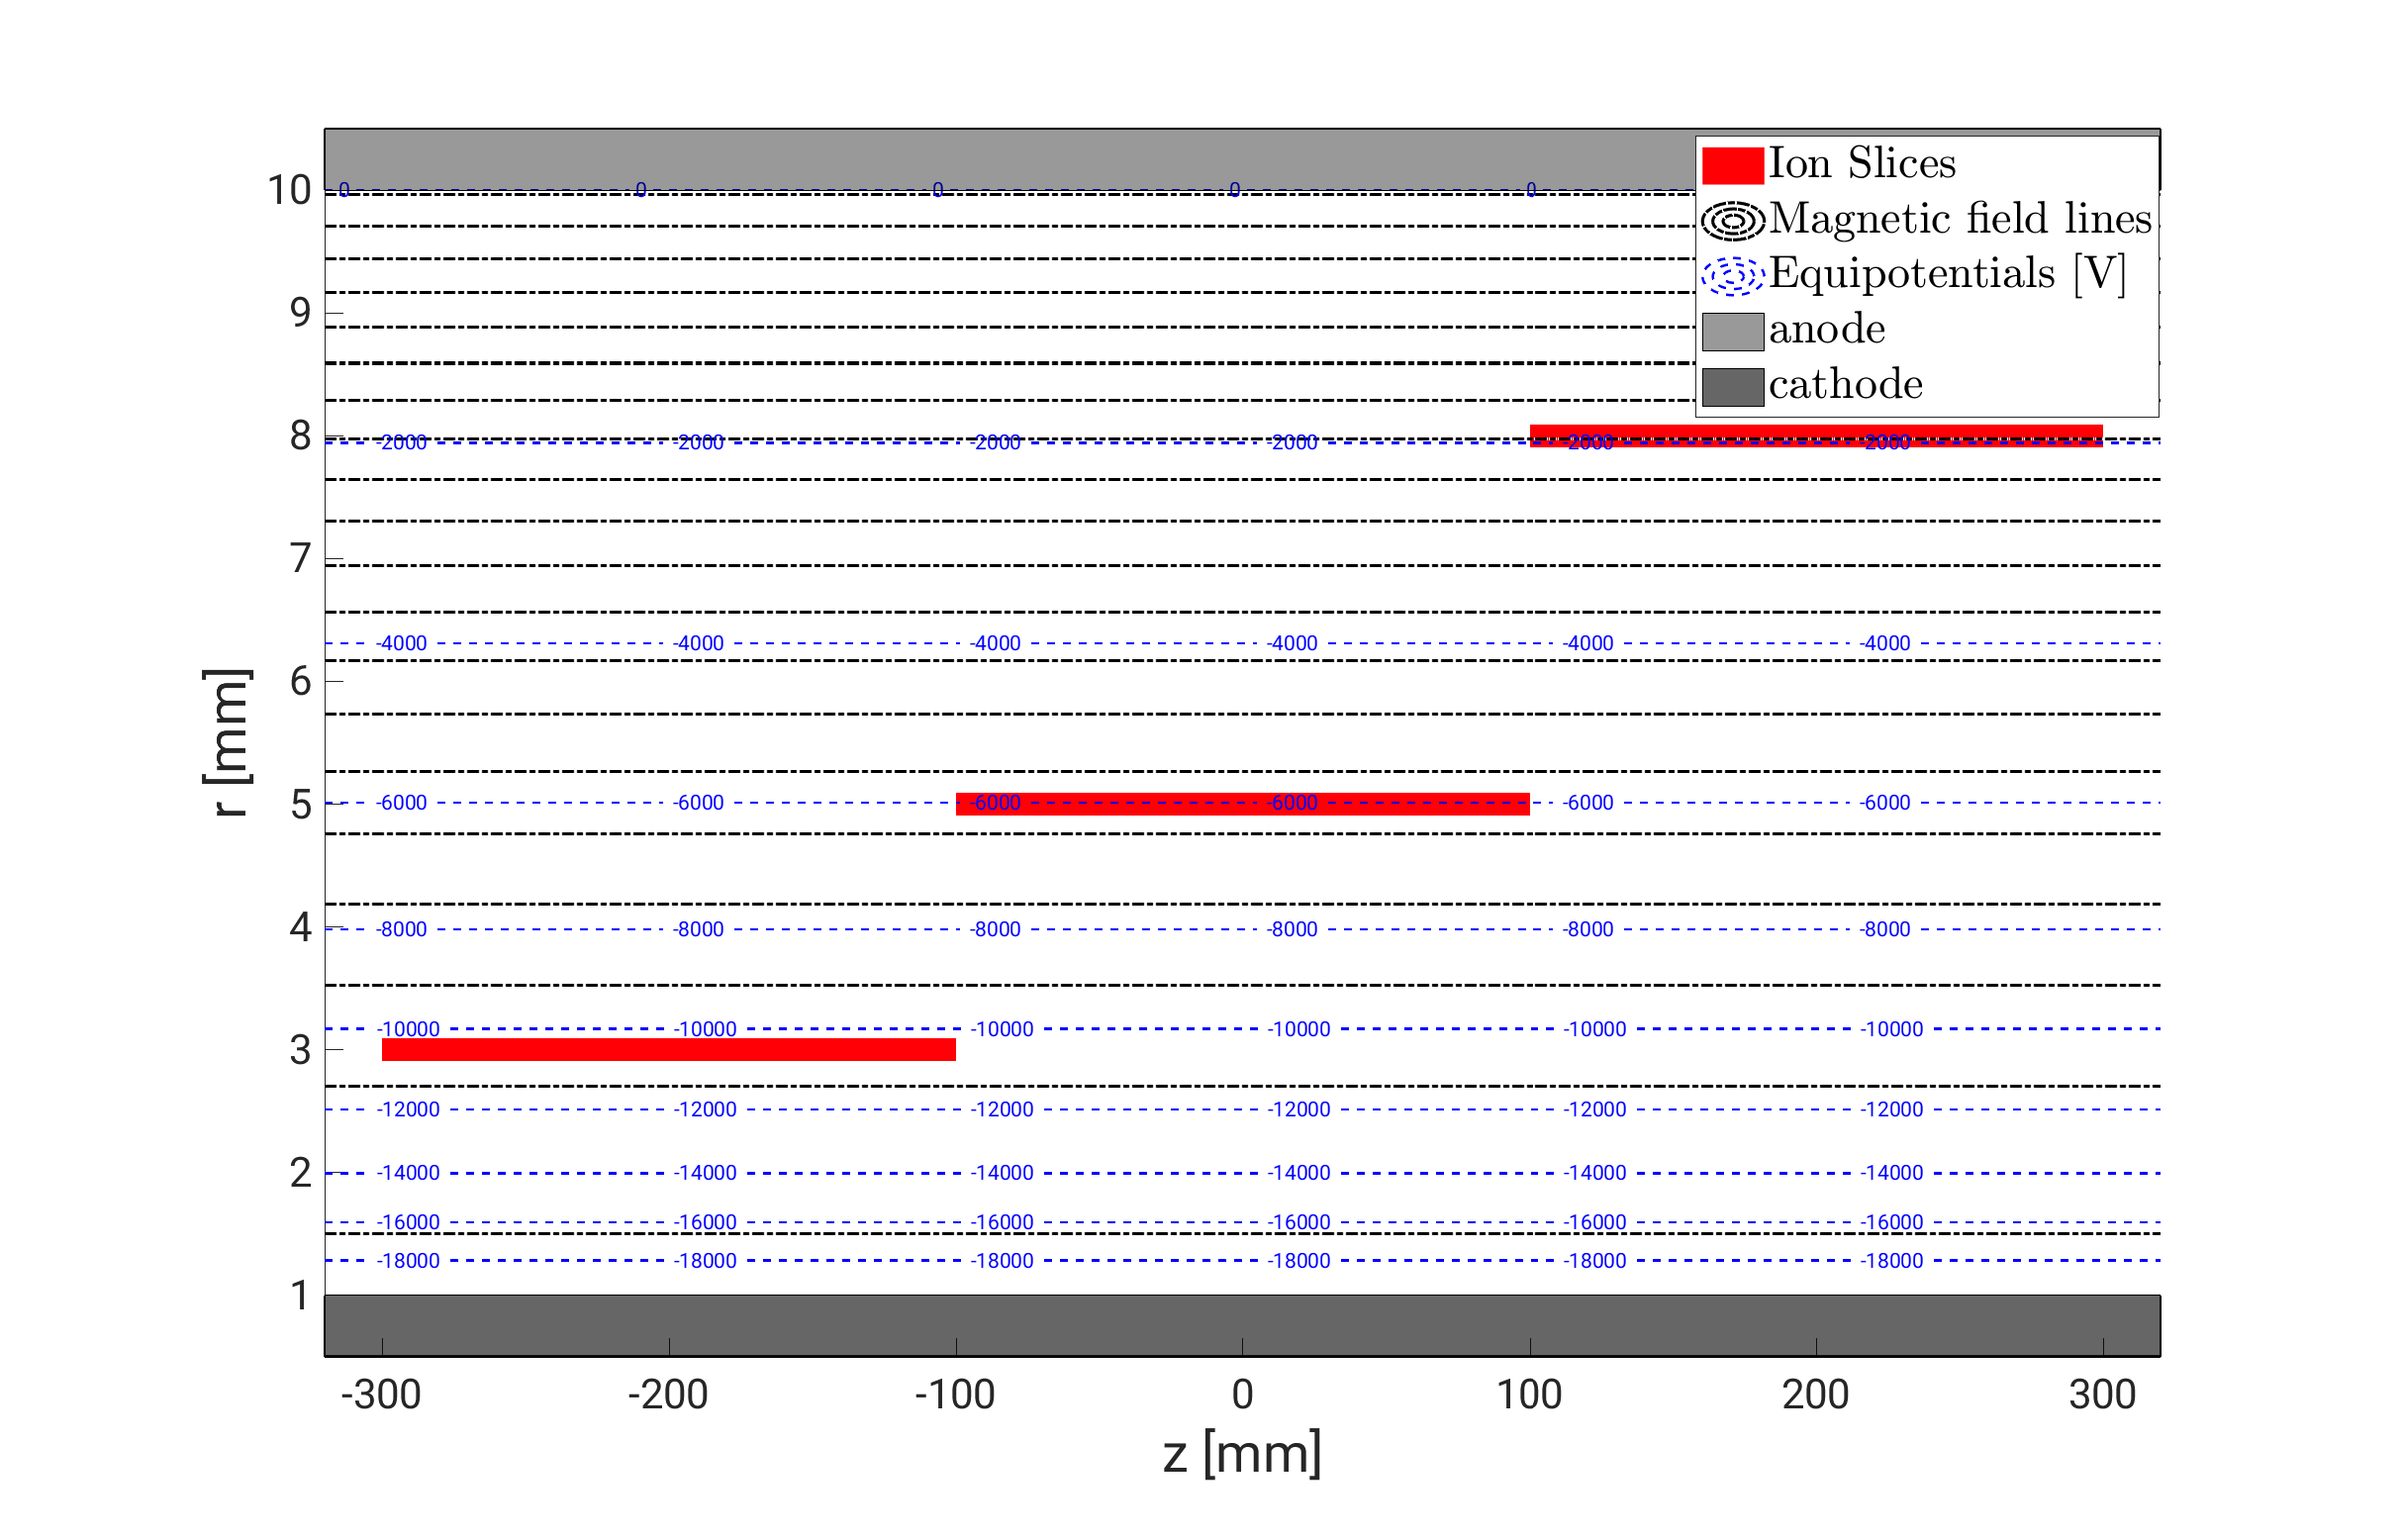
\includegraphics[width = 0.6 \textwidth]{FlatSlice_config.eps}
	\caption{\label{slice_config}  Initial ionic configuration used to produce the statistics from Table.(\ref{tab_stat}). The red stripes denote the initial ions positions. Note that by azimuthal symmetry, the ions are disposed on annuli. }
\end{figure}  

The statistical results presented in Table.(\ref{tab_stat}) are interesting in the sense that the theoretical model seems to have been implemented correctly. Regarding the relative errors, they are always lesser or equal to $1.6\%$, which is an acceptable value considering the fact that the model is approximative in several ways. Indeed, the yield conversion from $H^+$ to $H_2^{+}$ exposed in Eq.(\ref{Yield_H2+}) is an approximation. The fact that the yield in the potential emission region was constant (see Eq.(\ref{pot_em})), and that we linearly interpolated this constant value to the bottom of the kinetic emission model, constitutes one more source of approximation. However, this description is sufficient for a simple estimate of the influence of IIEE on electron clouds formation and behavior. Indeed, the yield being of the order of $\sim 1-2$, the approximations made should not influence or disturb greatly the expected results, in terms of electronic densities for example. \\

\begin{table}[h]
  \centering
  \renewcommand{\arraystretch}{1.2}
  \begin{tabular}{|p{5cm}|c|c|c|c|cl}
    \hline
    \center{\textbf{$^{304}$SS}}& $E_1$ & $E_2$ & $E_3$\\
     \hline
    $\gamma_{th}$ & 1.311  & 1.623 & 1.870  \\ \hline
    $\gamma_{iiee}$ & 1.299 & 1.627 & 1.891   \\ \hline
    $\epsilon_{rel}$ & 0.9\% & 0.2\% & 1.1\%  \\ \hline
     %----------------------------------------------------------------
    \center{\textbf{Cu}} & $E_1$ & $E_2$ & $E_3$ \\
     \hline
    $\gamma_{th}$ & 1.237 & 1.522 & 1.746   \\ \hline
    $\gamma_{iiee}$ & 1.229 & 1.518 & 1.760  \\ \hline
    $\epsilon_{rel}$ & 0.6\% & 0.3\% & 0.8\%  \\ \hline
     %----------------------------------------------------------------
     \center{\textbf{Al}}& $E_1$ & $E_2$ & $E_3$ \\
     \hline
    $\gamma_{th}$ & 0.920 & 1.133 & 1.297  \\ \hline
    $\gamma_{iiee}$ & 0.910 & 1.115 & 1.293   \\ \hline
    $\epsilon_{rel}$ & 1.0\% & 1.6\% & 0.3\%  \\ \hline
  \end{tabular}\caption{Yield statistics for H$_2^{+}$ ions impinging on the three materials}\label{tab_stat}
\end{table}

The last phase of the module testing was to determine wether or not some of the electrons generated by ions colliding with the electrodes would be kept in the simulation domain, or if no matter the geometry, they would be lost, as on Fig.(\ref{flat_slice}). To do so, an initial non-zero ion density was implemented in a region that was known to trap electrons, in a geometry where the cathode has half an ellipse dug inside it, as shown in Fig.(\ref{config_trapped}) - Left. This is one of the geometry planned to be mounted in the TREX experiment. No electron cloud was present at the time, so the potential well naturally present due to the topology of the $\mathbf{E}$ and $\mathbf{B}$ fields was not affected by the presence of an electron cloud. All the electrons produced at the electrode by IIEE were tracked down in a specific species in the code, so they would not be mixed up with the other electrons, coming from ionisations of the RNG. The right plot of Fig.(\ref{config_trapped}) shows the orbits of two among all the electrons that have not left the simulation domain. One notes that they were trapped in the potential well, bouncing at its axial limits, while they were drifting azimuthally over several full poloidal periods. The radial width of the orbit is defined by the Larmor radius. With this information in hand, it appears that ion induced electron emissions could produce interesting results regarding the formation of clouds. For example, the formation time could be influenced, the maximum density too. This will be treated in the next subsection.\\

\begin{figure}[h!]
\centering
	\includegraphics[width = 1.0 \textwidth]{config_trapped_rect.jpg}
	\caption{\label{config_trapped} Left: trapping region from the TREX extrude geometry. A cloud is present and the initial ion distribution is emphasized by the blue rectangle. - Right: vacuum potential well and two trapped electrons orbits.}
\end{figure}  

\subsection{Cloud formation}

Now, let us deal with results concerning the clouds formation and dynamic, with and without taking account for IIEE. In first considerations, two particular TREX geometries have been implemented. Let us start with results in the \emph{slanted} geometry, that is with a prominent half-ellipse coming out of the anode, as in Fig.({\ref{TREX_schematics}}).\\

\textbf{TREX \emph{slanted} geometry}\\

Several characteristics are of interest in this case. As mentioned before, the characteristic time of cloud formation might be affected by the IIEE. The peak cloud density could also be increased. It can be interesting to look up the currents present at the boundaries too. Indeed, a strong electric current is as much as the source will not have to supply. To obtain these informations, two situations are considered. The geometry is the same for both, that is with the ellipse protruding from the anode. The anode is grounded, and the cathode is at $\Phi = -20$ kV. The magnetic field intensity is of about $B = 1.15$ T on the high field side (low $z$), and decreases down to $B=0.15$ T on the low field side (high $z$). The magnetic field topology and the initial electronic configuration are shown together in Fig.(\ref{Config_mag_Slanted}). Since the bottom of the ellipse is know to be a trapping region, a rectangle distribution of electrons is initialised below it, in order to act as a source of ionisation, to produce the ions by collisions with the RNG. Now two cases are to be distinguished: the case with and the case without IIEE.\\

\begin{figure}[h!]
\centering
	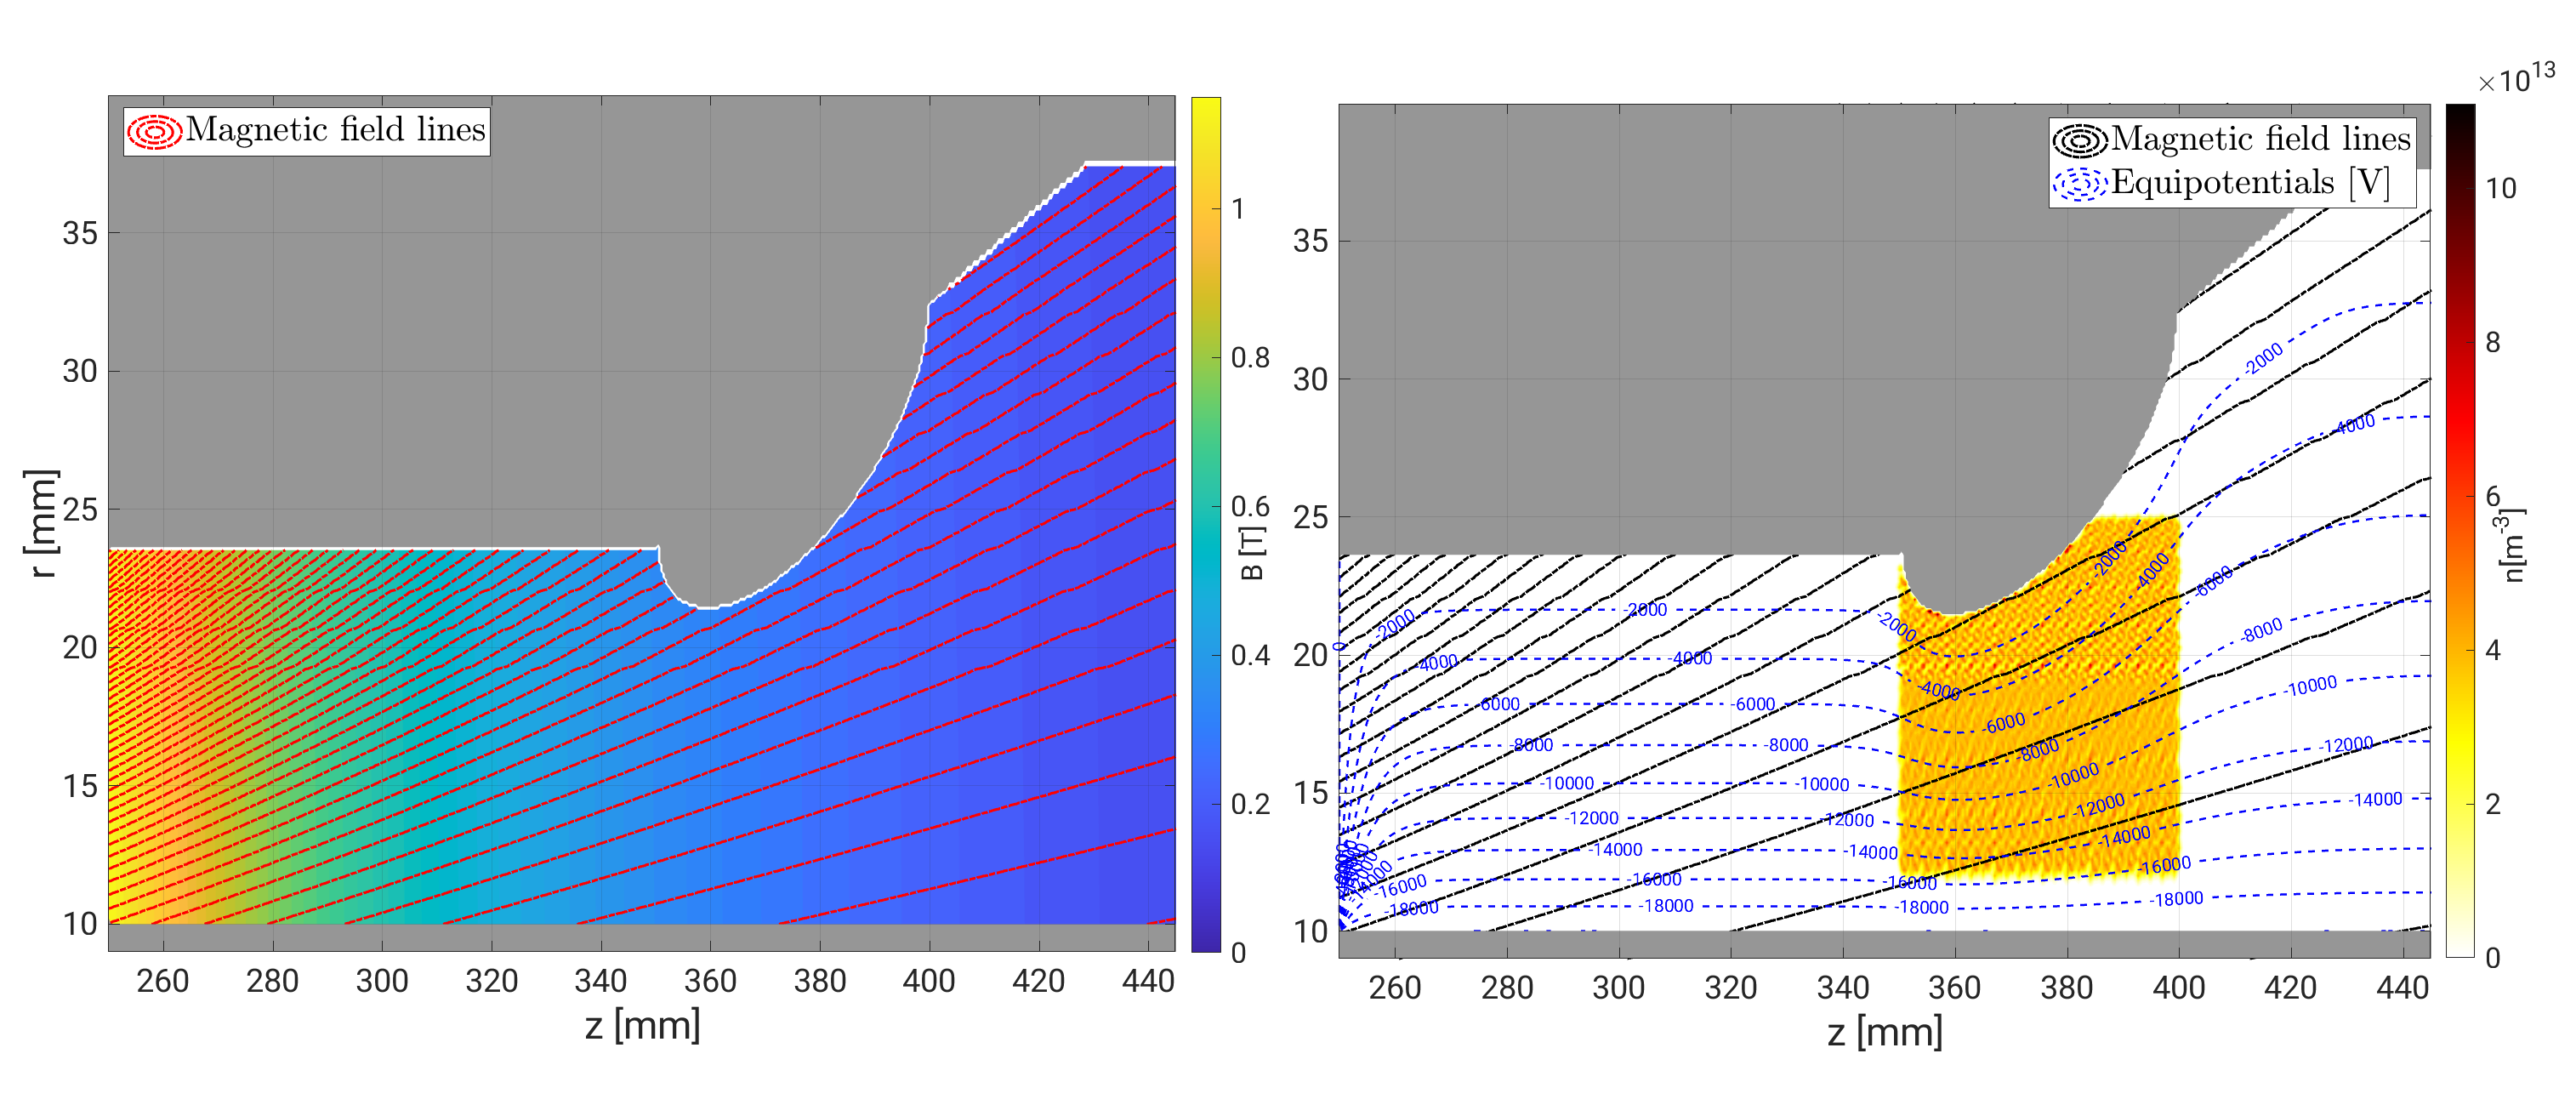
\includegraphics[width = 1.0 \textwidth]{Config_H2Slanted.eps}
	\caption{\label{Config_mag_Slanted} Left: magnetic configuration from the TREX slanted geometry. - Right: initial configuration of electrons, leading to the formation of an electron cloud.}
\end{figure}  


Let us first compare how fast the steady state is reached in both situations. Recall that the steady-state is characterized by the ions loss equal to the electrons loss. Hence, this is supposed to imply that the ionic current and the electronic current are constant over time, and of the same order of magnitude. Regarding the number of particles, it is supposed to reach a maximum and stagnate. The time required to reach this maximum corresponds to the cloud formation time. Plotting the total electronic charge over time can be a great indicator of the state of formation of the cloud. It can also enable to compare the formation in the two situations, where IIEE are considered and not. \\

\begin{figure}[h!]
\centering
	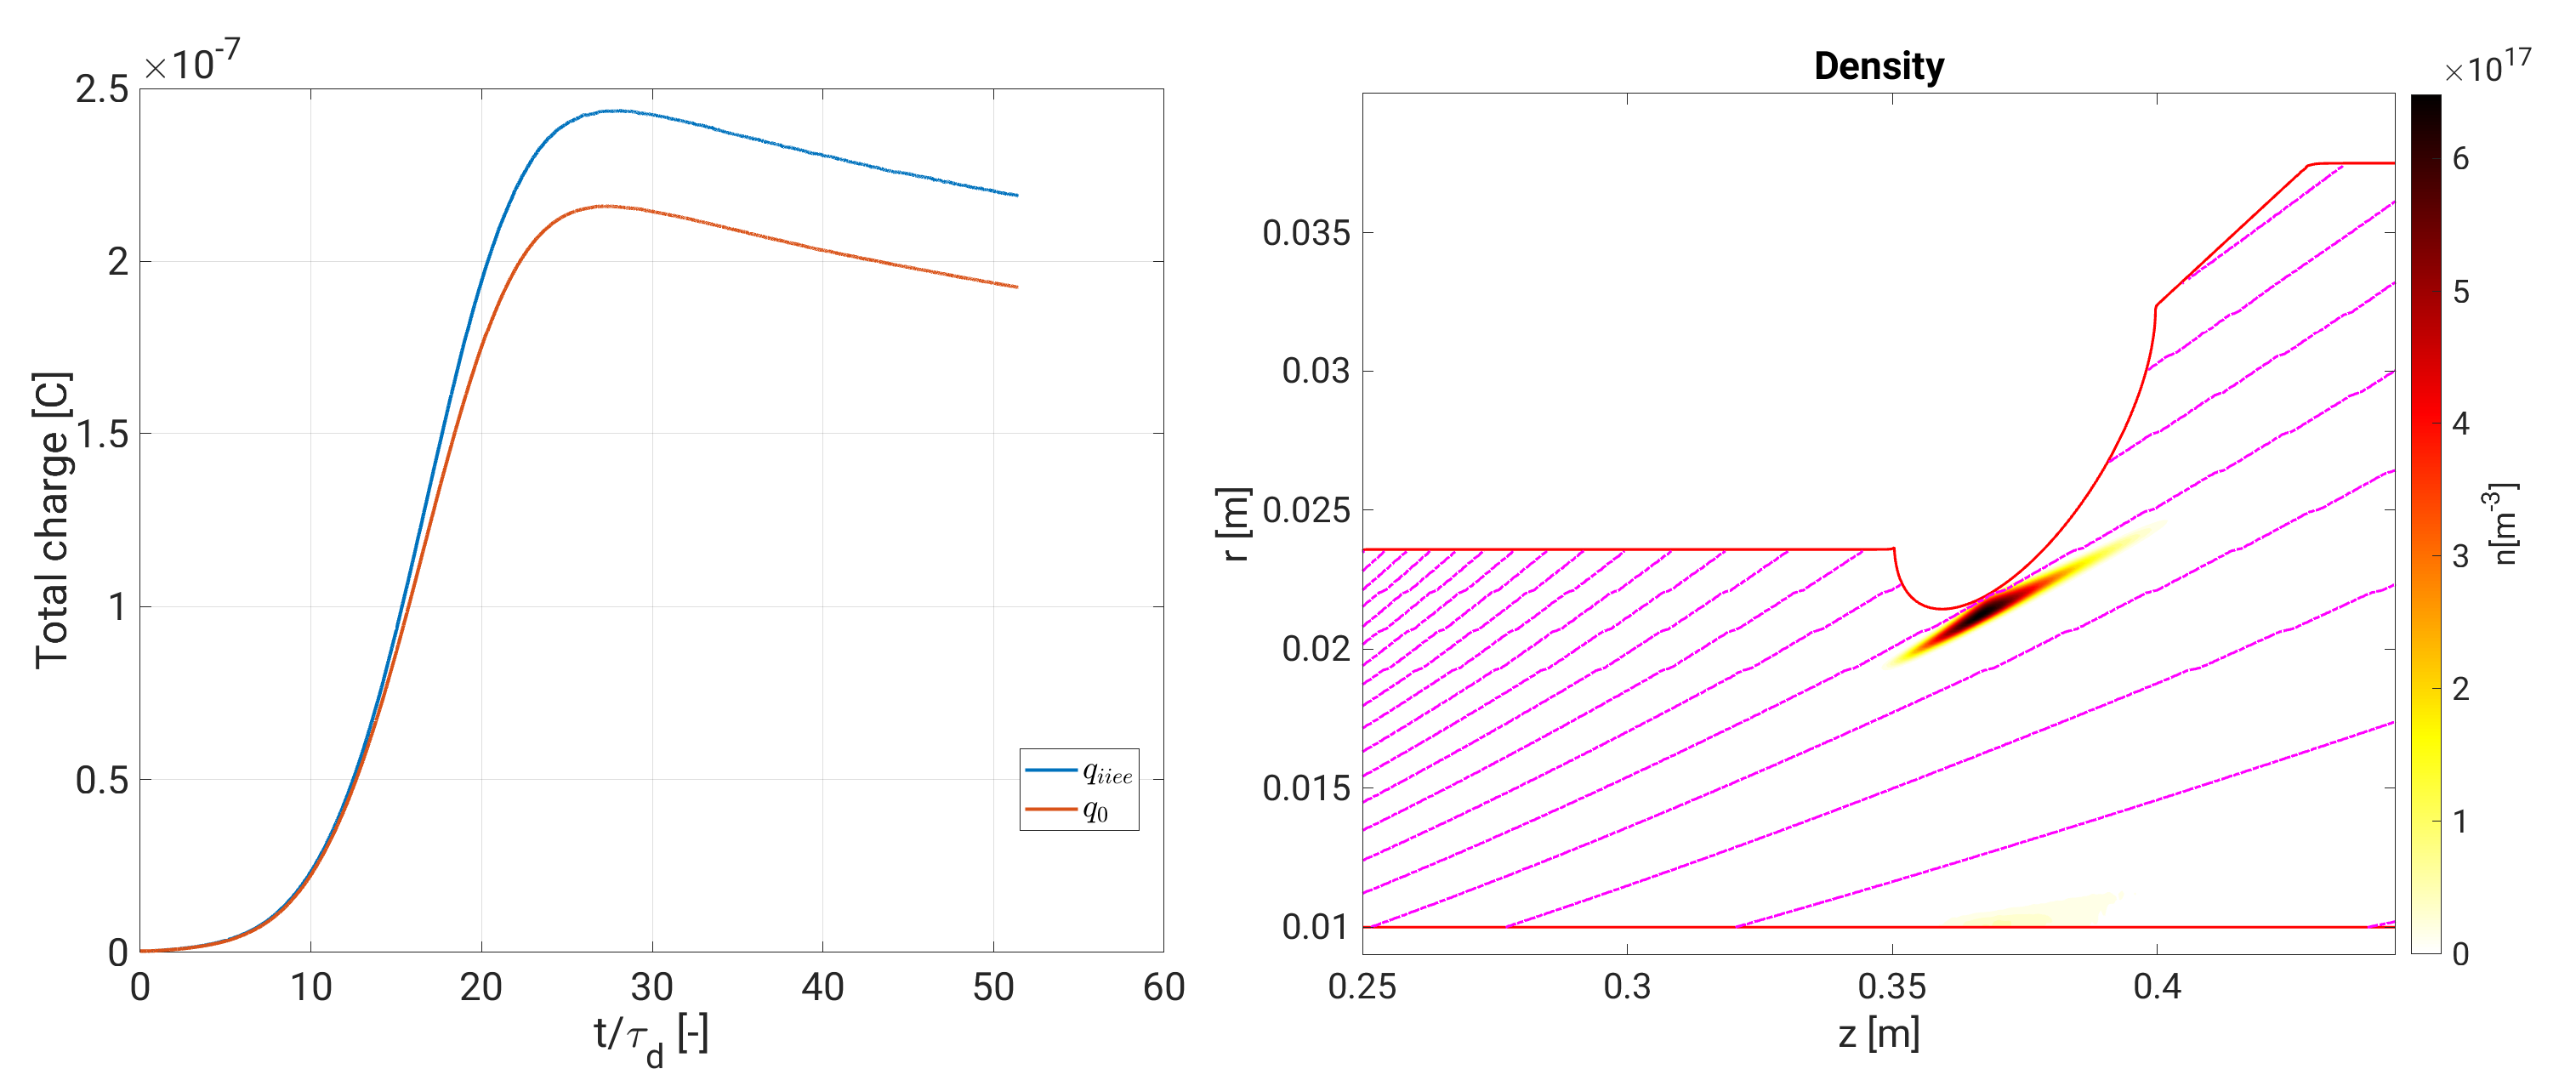
\includegraphics[width = 1.0 \textwidth]{elec_density_current.eps}
	\caption{\label{elec_density_current} Left: evolution of the total electronic charge inside the domain, over time normalised by the collision time. - Right: electron density in steady state.}
\end{figure}  

On the left part of Fig.(\ref{elec_density_current}), the absolute value of the total electronic charge in the domain is represented over time, the time being normalised by the collision time, to remove the pressure dependency. The blue curve represents the charge when the ion induced emissions are taken into account. One notes that the formation times are similar, since the inflexion point of each curve is located at about the same time, and so is the peak value. As expected the charge is higher, since more electrons have been produced. Note that this information alone is not sufficient to determine wether the total charge is higher because more electrons have accumulated in the cloud, or if they are present elsewhere in the domain. This is why the electron density is plotted in steady state, on the right plot of Fig.(\ref{elec_density_current}). Although it is not represented, both clouds, with and without IIEE had the exam same density and shape (hence, for the sake of saving space, only the situation with IIEE has been shown). This is consistent with our expectation, since the ion-induced electrons are formed at the cathode, and the potential well is located right by the anode. It is clear that these electrons, due to their Larmor motion along field lines, cannot reach the cloud and be trapped too. They will simply leave the domain axially, and contribute to a source of axial current. Now, one question arises: what is the order of magnitude of this ion-induced electronic current ?\\ 

To answer this question, the current collected at all the boundaries of the domain has been plotted over time. The boundaries are the axial limits, $z=250$ mm and $z=445$ mm, and the metallic electrodes. The curves shown in Fig.(\ref{TotCurr_less}) corresponds to the currents collected in the case where the IIEE were not considered. The purple curve corresponds to the electronic current collected in the region of the ellipse, as the cloud is progressively compressing against the electrode and leaking electrons towards the metal. The plain green line corresponds to the electronic current at the cathode, which is consistently approximately zero. The green dashed line corresponds to the ionic current at the anode, while the yellow plain line shows the axial current at the low field side, that is electrons leaking from the potential well as it is progressively squeezed against the anode (see Fig.(\ref{pot_well_all}) for the evolution of the potential well). The black plain curve represents the total current, that is the sum of all these contributions. The dashed black curve corresponds to the sum of all currents from Fig.(\ref{TotCurr_H2}), for the sake of comparison. The blue (plain) line shows the evolution of the electron density $n_e$ over time, in order to visualise when the steady state is reached, while the dashed one corresponds to the electrons density in the lower radial half of the domain. Note that the time has been normalised here by the collision time $\tau_d$. As predicted, in steady state, the ionic (dashed green) and electronic (purple + yellow) are constant  and of the same order. Of course, no current is collected on the high field side. \\

\begin{figure}[h!]
\centering
	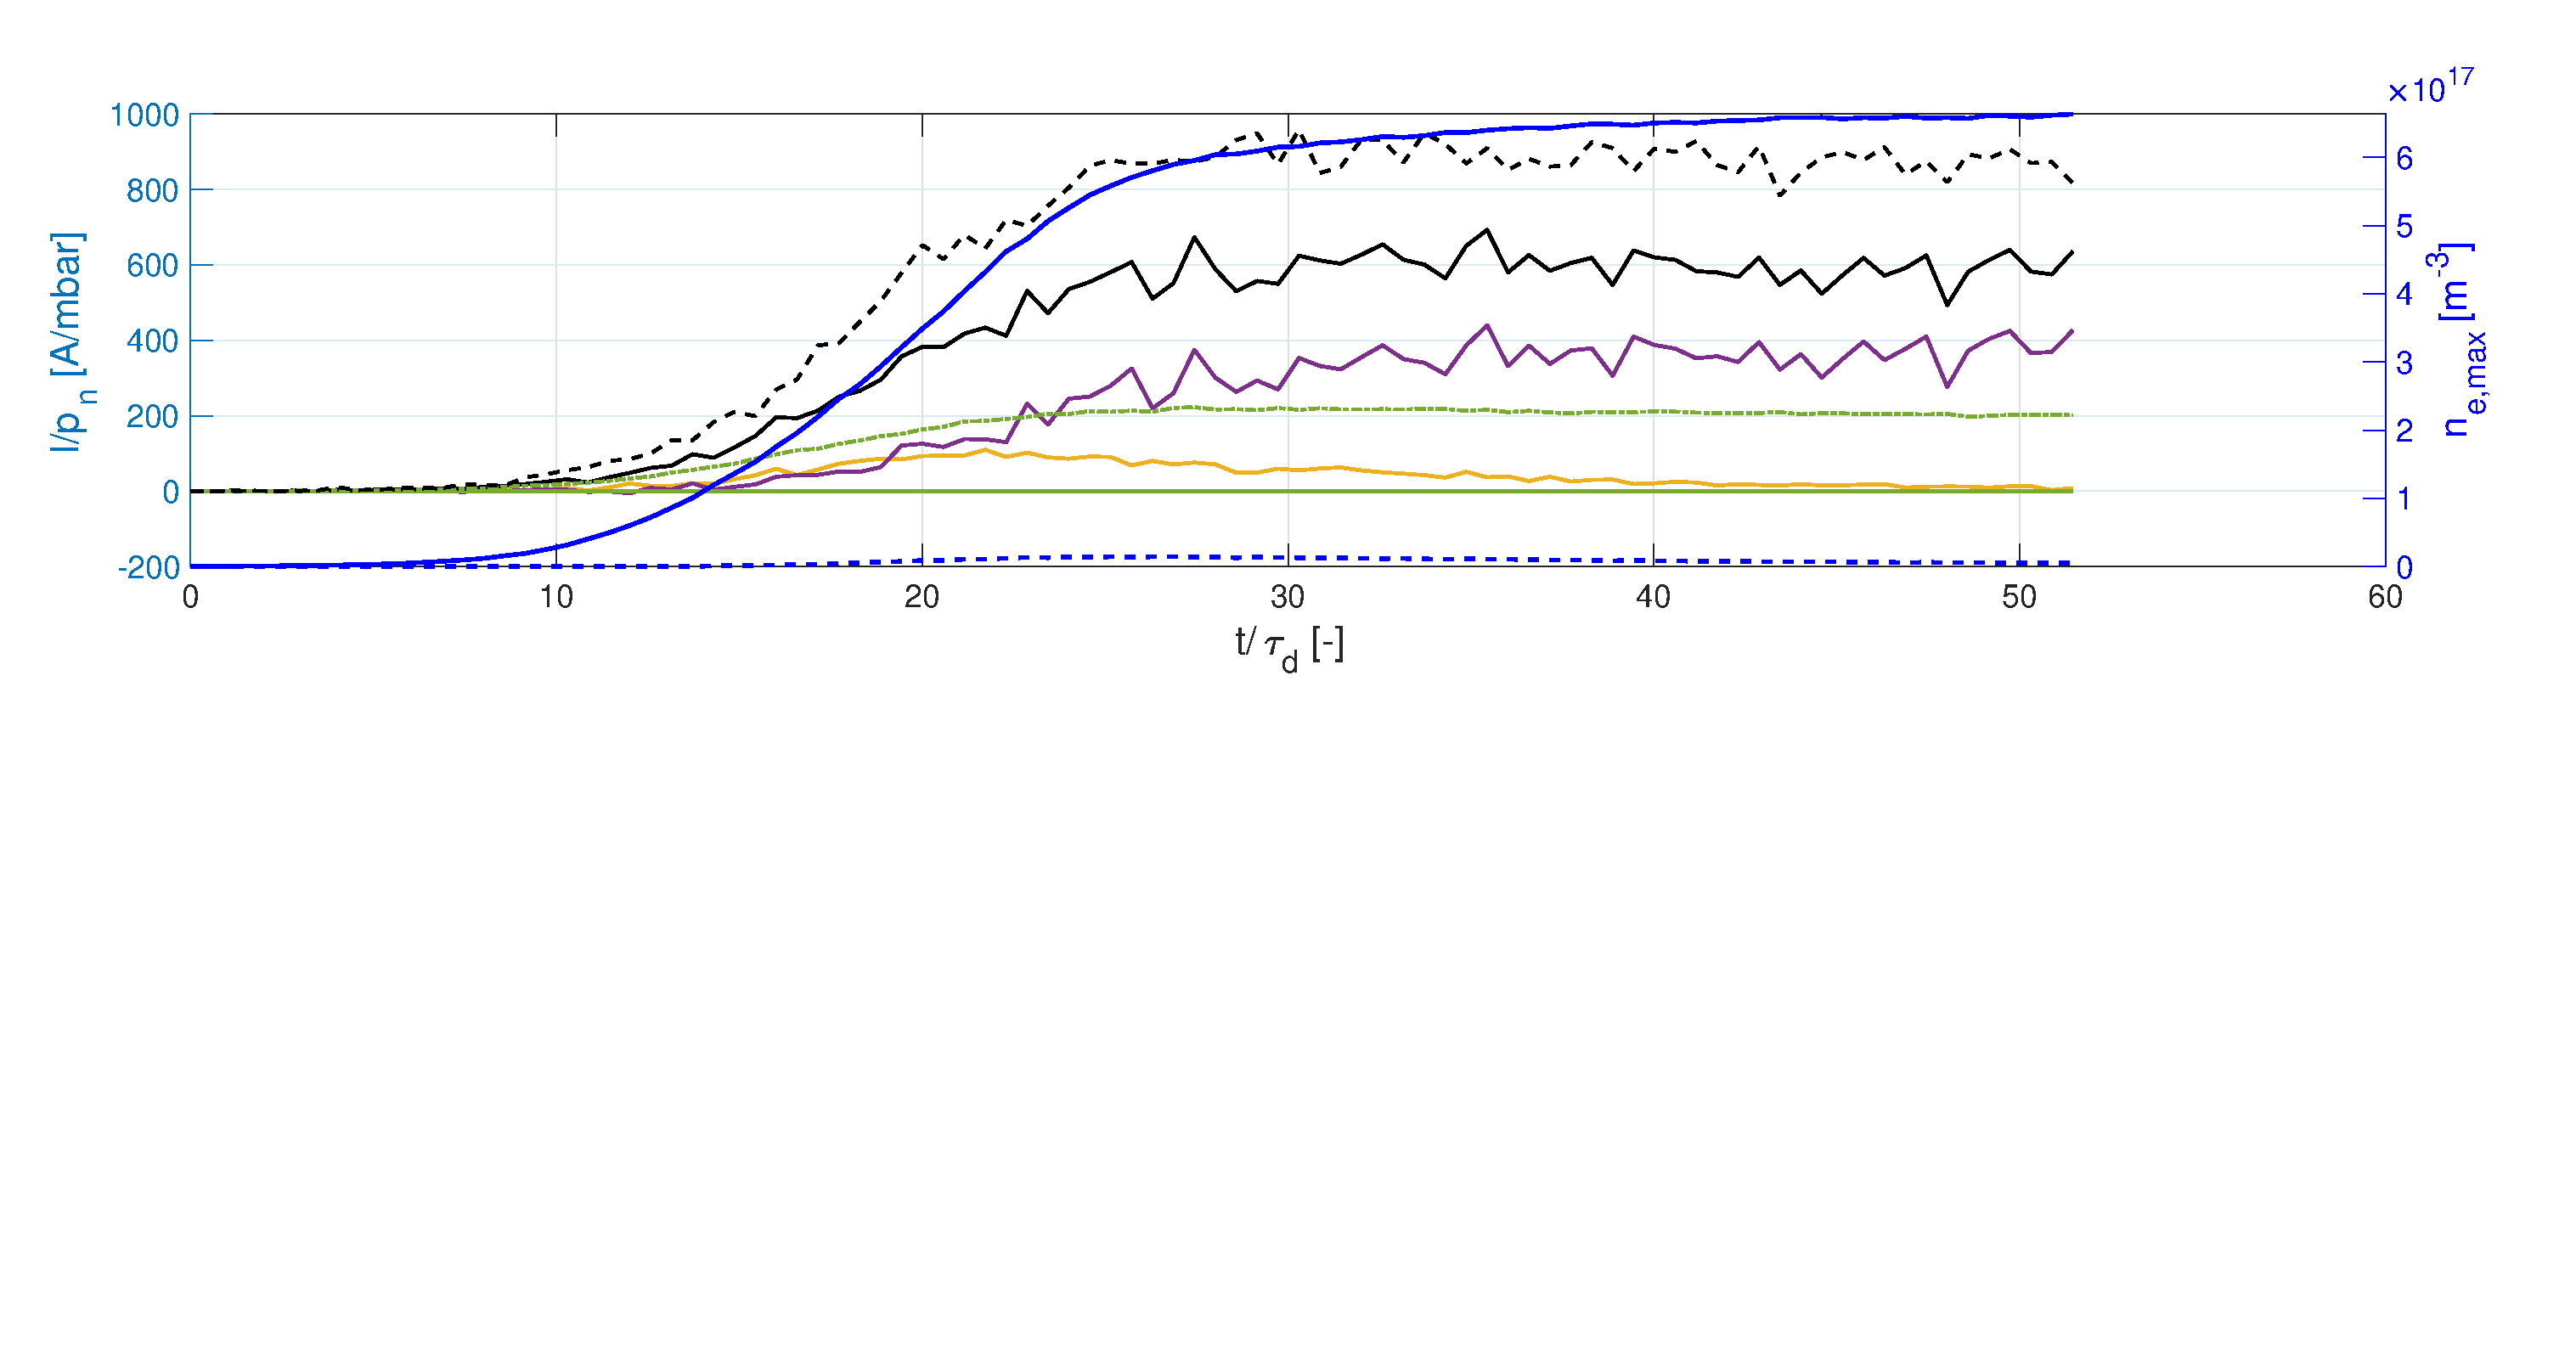
\includegraphics[width = 1.0 \textwidth]{TotCurr_less_onlycur}
	\caption{\label{TotCurr_less} Currents collected at all the boundaries of the domain, in absence of ion induced electron emissions. The colors correspond to the domains highlighted at the bottom part of  Fig.(\ref{TotCurr_H2})}
\end{figure} 

\begin{figure}[h!]
\centering
	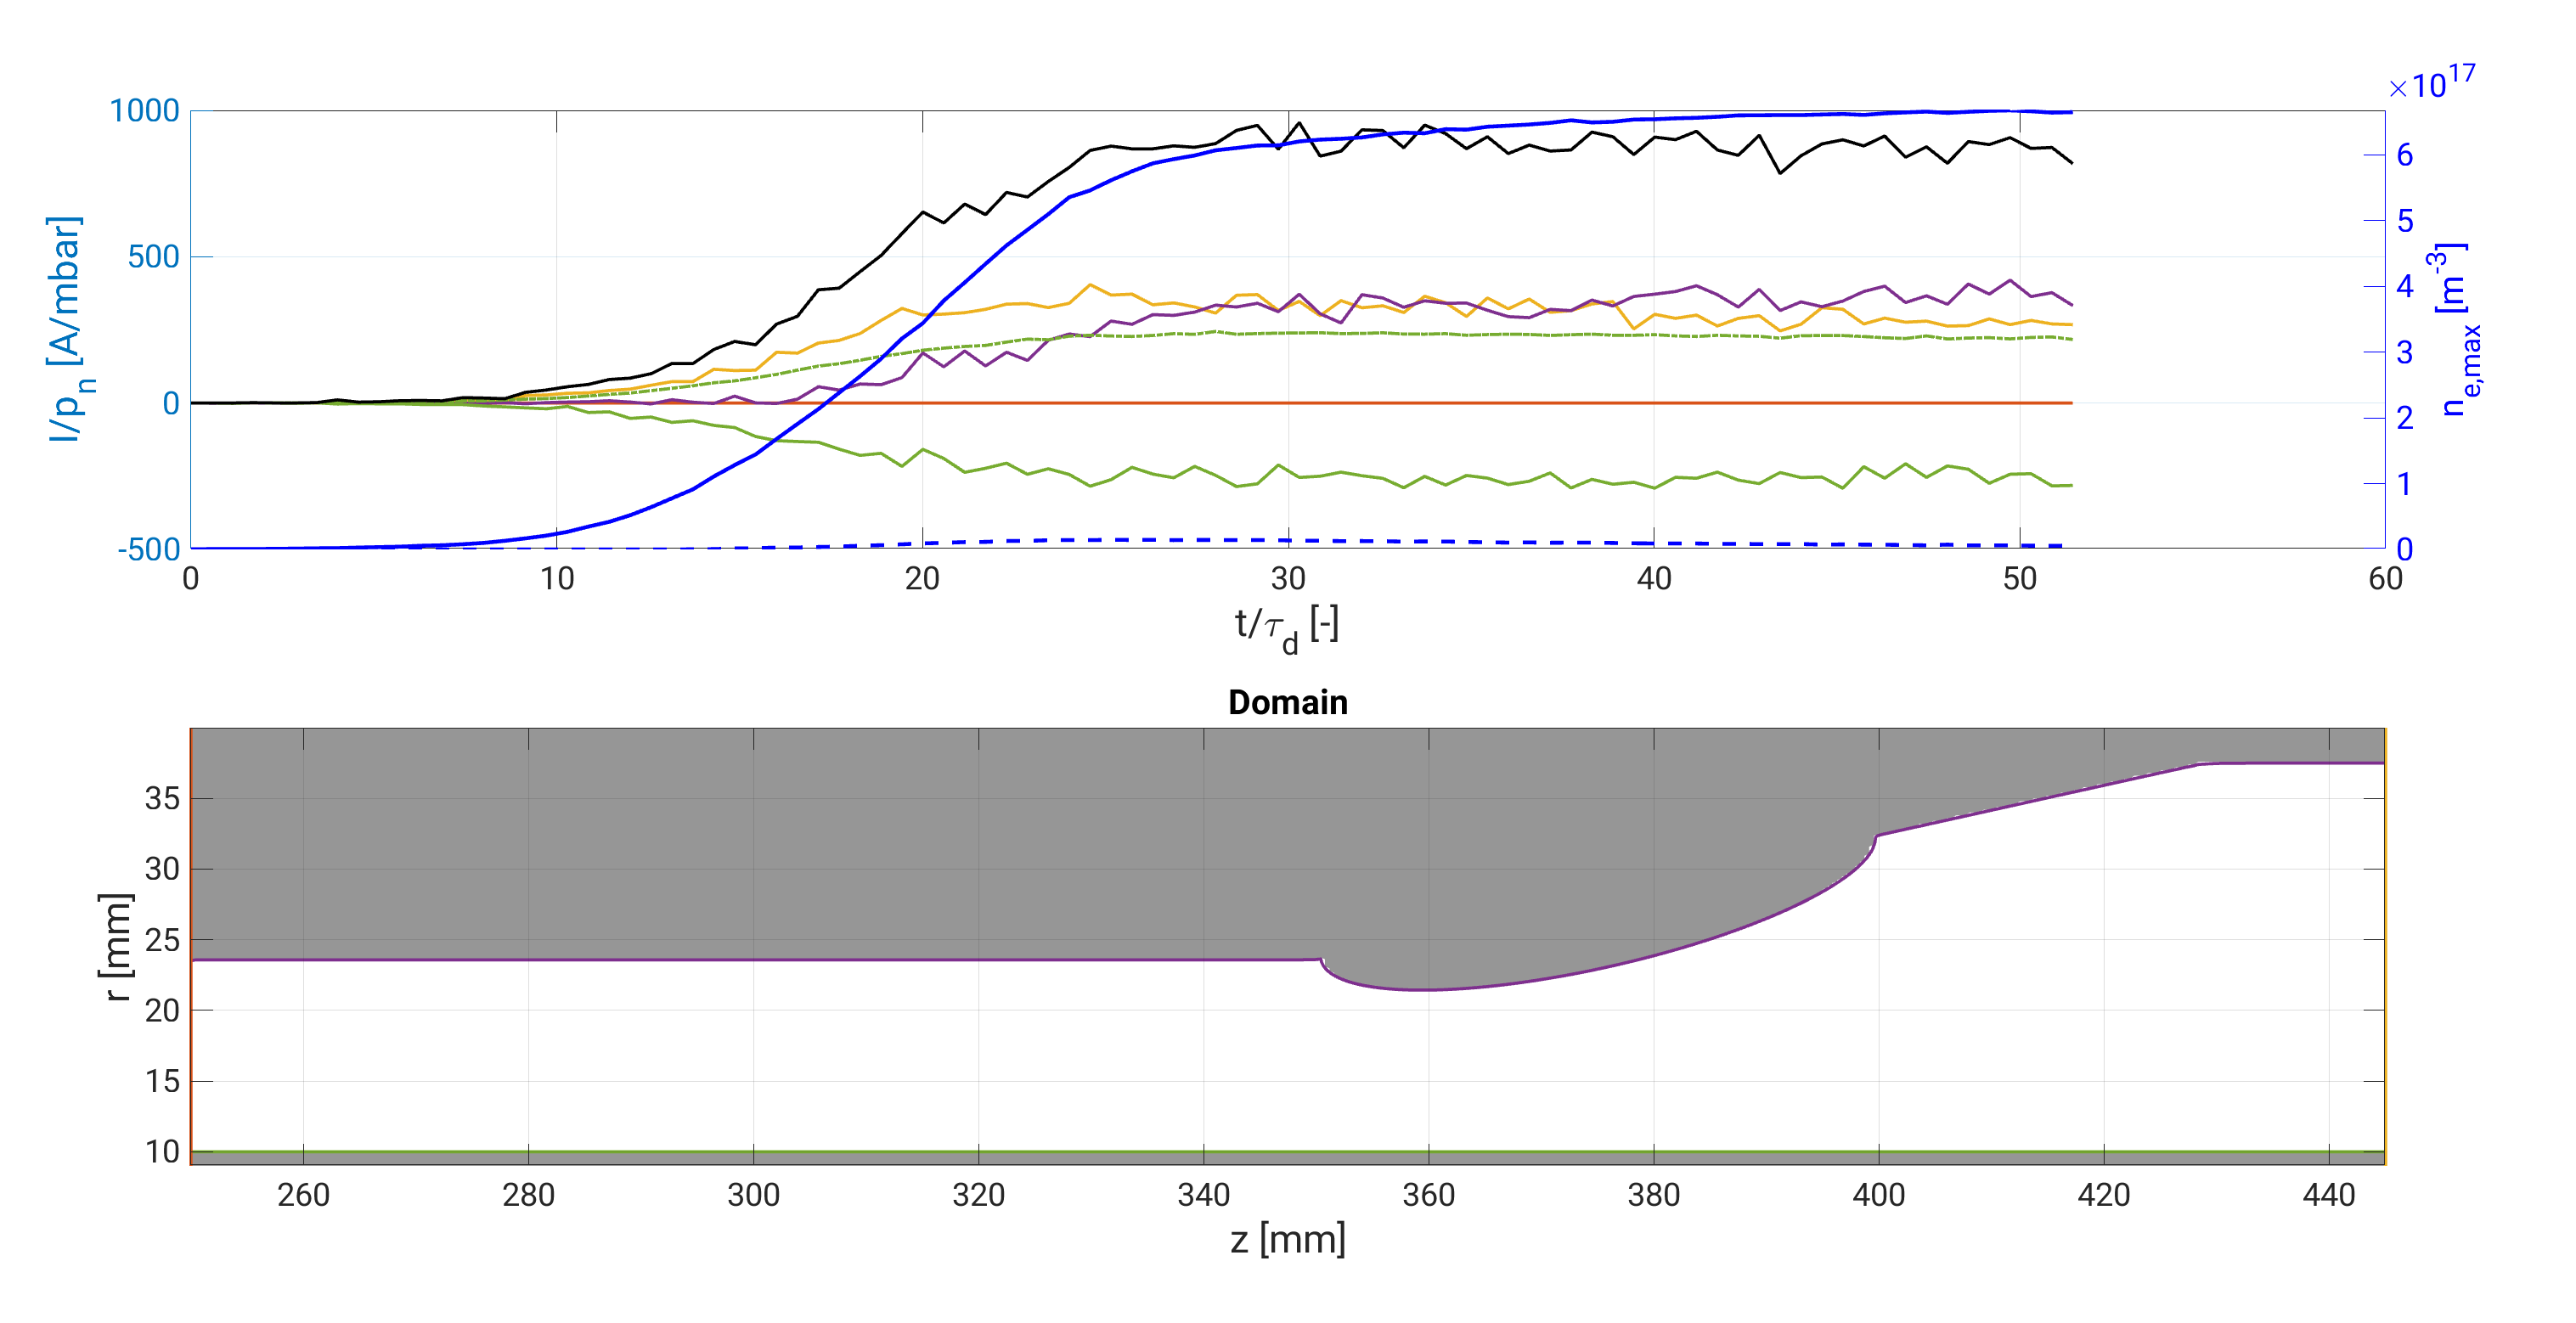
\includegraphics[width = 1.0 \textwidth]{TotCurr_H2_iiee.eps}
	\caption{\label{TotCurr_H2} Top: Currents collected at all boundaries of the domain, taking account for IIEE. - Bottom: Domain and boundaries definitions. The high field side is in red on the left, the low field side in yellow, the cathode in green and the anode in purple.}
\end{figure} 

The high plot from Fig.(\ref{TotCurr_H2}) represents the same information as in Fig.(\ref{TotCurr_less}), with the exact same color code. However, the contributions to the different currents might change a little bit. Still, no current is collected on the high field side. The electronic current collected at the anode is approximately the same in both situations, emphasising that the cloud behavior does not depend on IIEE in this geometry. However, now a contribution (negative) of the total current at the cathode is present (green, solid line). This contribution is due to the electrons leaving the cathode as they are produced by the ions. Note that since the yield is on average, of the order of 1-1.5, the ionic current (green dashed) is approximately equal and of opposite sign as the electronic current leaving the cathode. The generation of electrons at the electrode being discrete events, the currents fluctuates a bit more around its average value. \\

\noindent Since the ions and the electrons have opposite charges, and they flow in opposite directions, the negative current at the cathode, coming from the electrons, will contribute to a new net current towards the grounded region. Indeed, all electrons being generated at the cathode are flowing towards the low field size to leave the domain. Thus, it is expected that the axial current is at least as important as the electronic current induced by electrons leaving the cathode. It turns out that it is even greater, since it contains the contribution from the electrons that are leaking from the cloud, see yellow line on Fig.(\ref{TotCurr_less}). The total current flowing from the cathode (at $\Phi = -20$ kV) to the grounded regions (low field side and anode), plotted in black, is now much greater than the total current observed without ion induced emissions. \\

\begin{figure}[h!]
\centering
	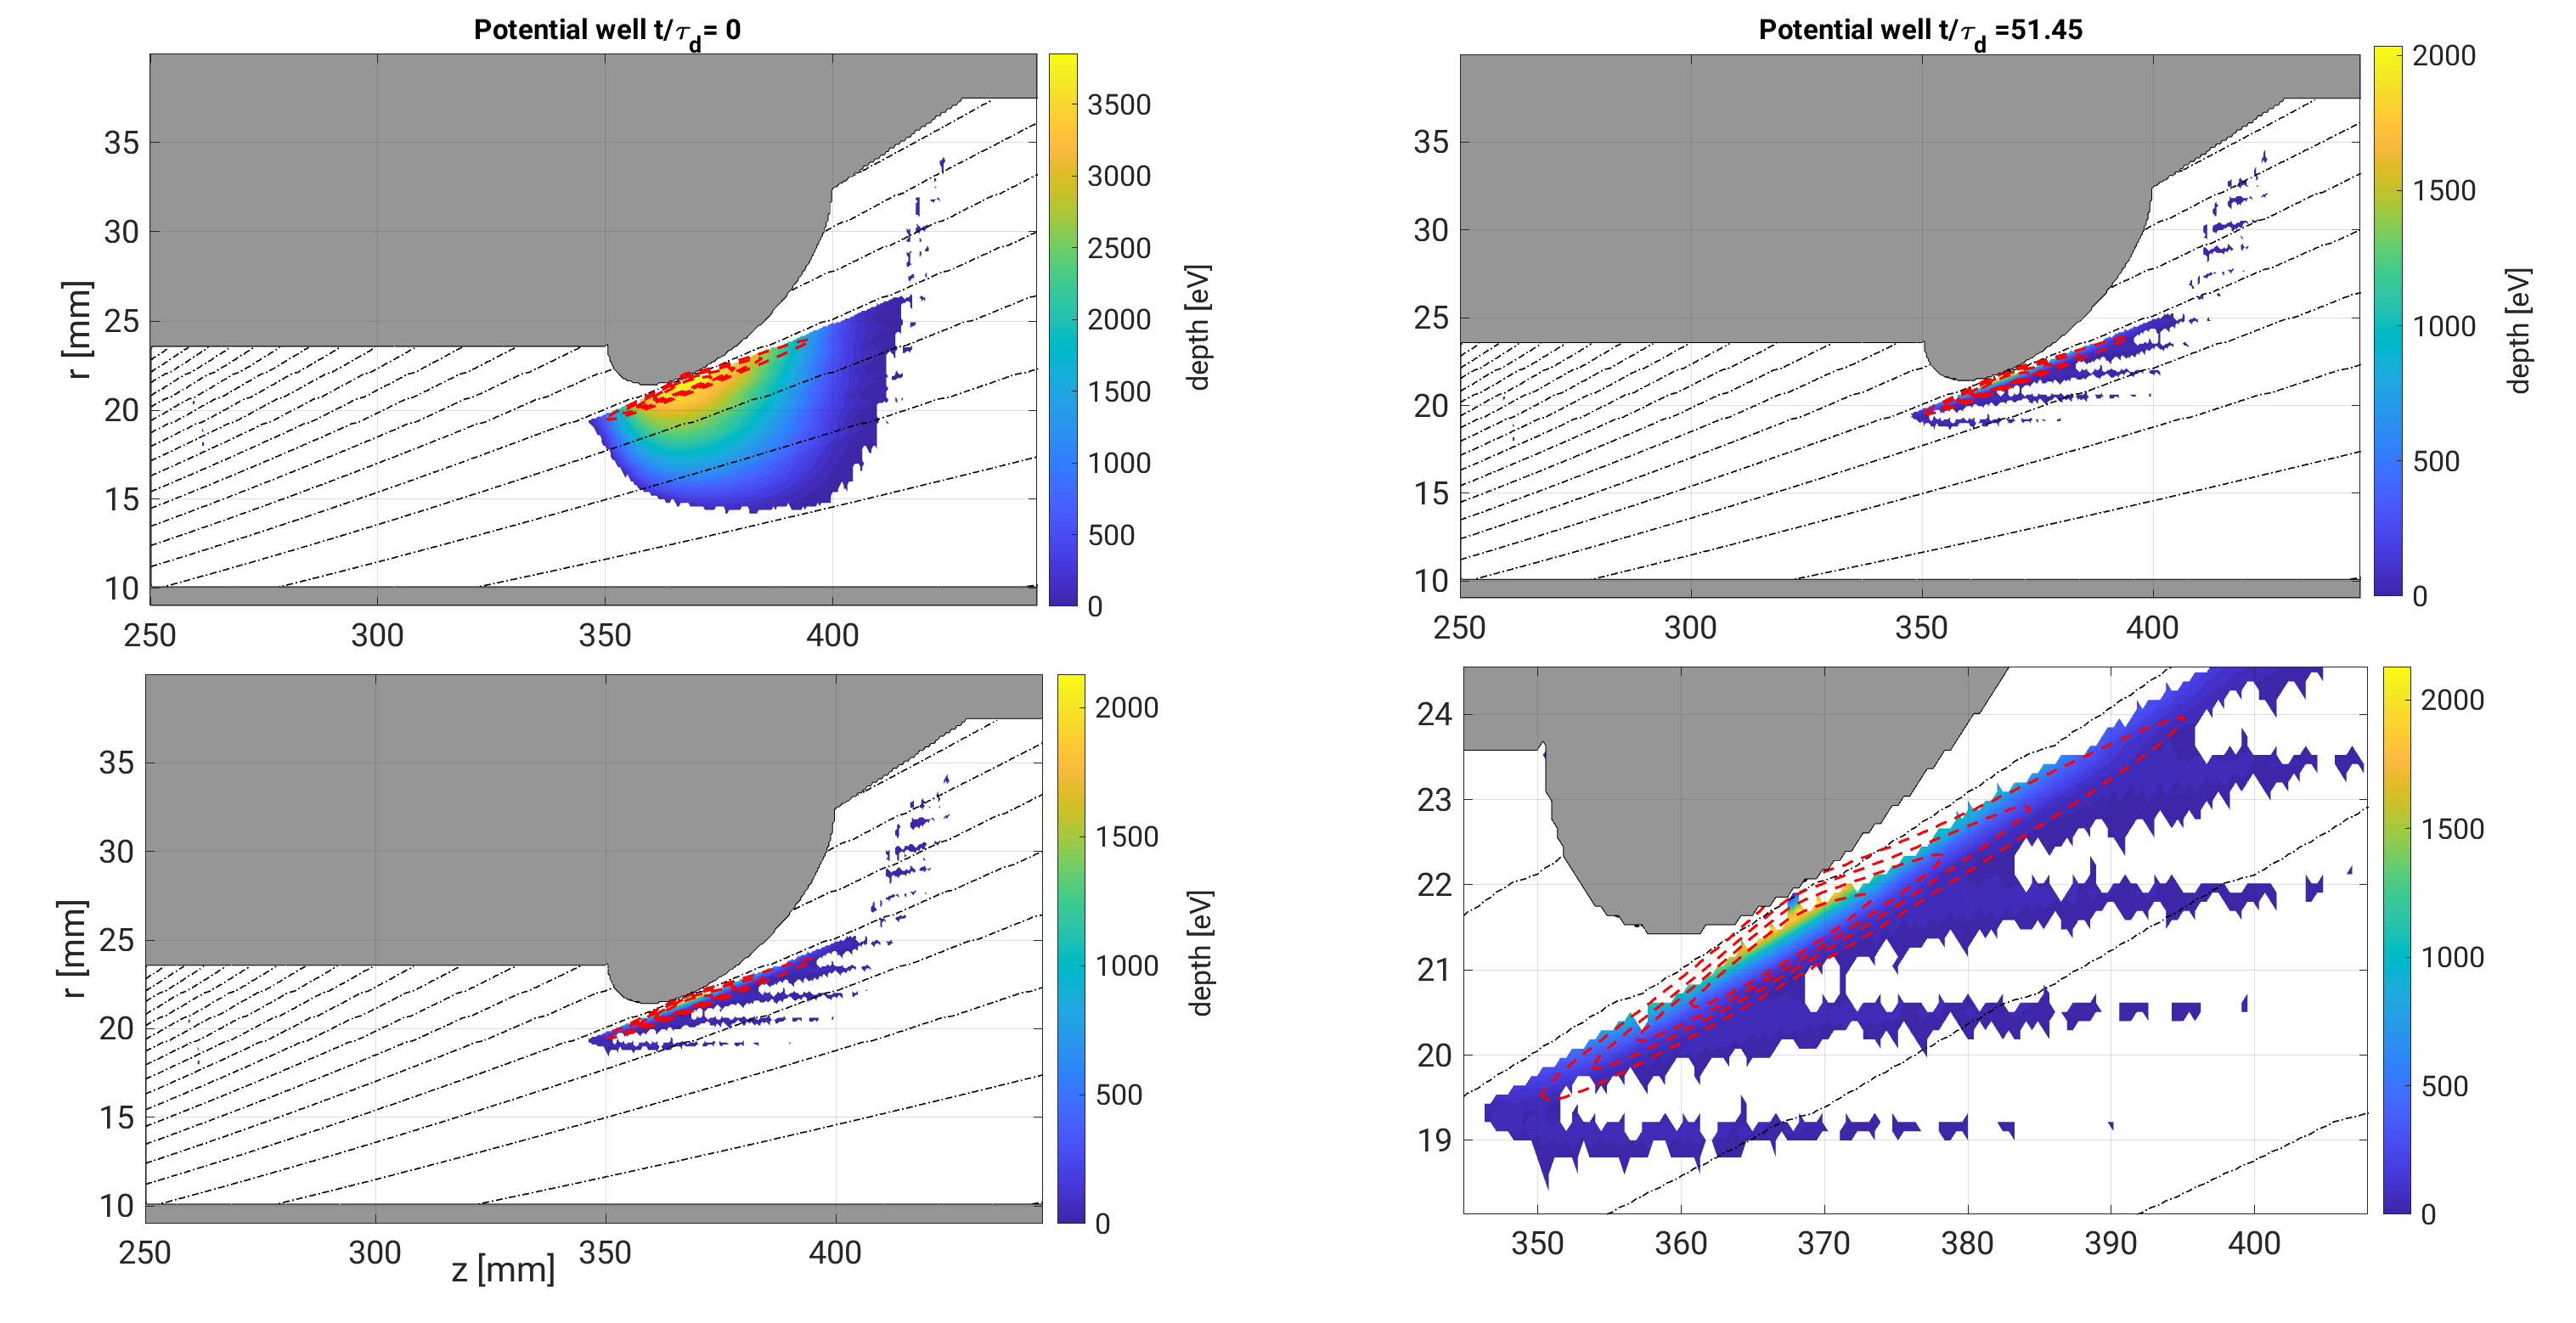
\includegraphics[width = 1.0 \textwidth]{Potential_well_all.eps}
	\caption{\label{pot_well_all} Potential well dynamics as the electron cloud forms. Up Left: Vacuum potential well - Up Right: Potential well in presence of the cloud (IIEE) - Down Left: Potential well in presence of the cloud (without IIEE) - Down Right: Zoomed view}
\end{figure}

\noindent The dynamic of the potential well as the cloud is forming is shown in Fig.(\ref{pot_well_all}). The upper left corner plot shows the vacuum potential well, that is the well formed naturally by the magnetic field line crossing the equipotentials, in absence of the cloud. For the sake of readability, the equipotentials have not been shown. The dashed red contours show where the cloud forms inside the potential well. The upper right and lower left corners plots show the potential well in presence of the cloud, with IIEE and without them respectively. Note that the wells are identical, as expected from the previous considerations. The lower right corner plots shows a zoomed view of the potential well, with the contours ouf the cloud. Note that the outer contour intersects the anode, explaining the purple curve in Fig.(\ref{TotCurr_less}-\ref{TotCurr_H2}), since some electrons from the cloud are collected at the anode. The potential well depth is remarkably affected by the cloud (see colorbar).\\

So to sum things up, the IIEE in this particular geometry seem not to influence neither the cloud formation time, nor the density. The clouds behave the same both with and without the ion induced electrons. As said previously, this can be explained by the magnetic topology, preventing the electrons leaving the cathode to reach the cloud's potential well. However, it is important to note that the electrons produced by the ions contribute to a non-negligible net current component, that adds up on top of the other contributions, coming from the cloud leaking electrons, and the ions. Hence, this new contribution has to be taken into account in the dimensioning and the design of the power supply for the MIG. \\
 
\textbf{TREX \emph{extrude} geometry}\\

Now, let us focus on one of the other designed geometries for TREX, the so called \emph{extrude} geometry, that is with half an ellipse dug inside the cathode. The electrode geometry has been shown previously in Fig.(\ref{extrude_config_both}). Here again, the anode is grounded, and the cathode is set at the potential $\Phi = -20$ kV. The magnetic field intensity is the same inside the domain, and designed to reproduce the field from a superconducting magnet outside the domain, on the high field side. In the region of the ellipse, $B$ ranges $\sim 0.35 - 0.22$ T. The vacuum potential well, as defined previously, is shown in the right plot of Fig.(\ref{extrude_config_both}). This ellipse aims at reproducing the bottom part of the trapping region, under the corona ring from a typical MIG, as shown in the dashed red region from Fig.(\ref{gyrotron}). It is also located in the same axial region as the outer ellipse form the \emph{slanted} geometry studied above, in order to be able to combine the two geometries, to be closer to the full MIG shape. However, splitting the study in two makes it easier to identify the physical phenomena influencing the formation of the clouds, and to separate the currents components. Indeed, taking the geometry where both the inner and the outer ellipses are present would lead to two clouds, preventing us from determining easily which cloud is responsible for which current and so on. Nevertheless, this would be the object of an interesting further study. \\


\begin{figure}[h!]
\centering
	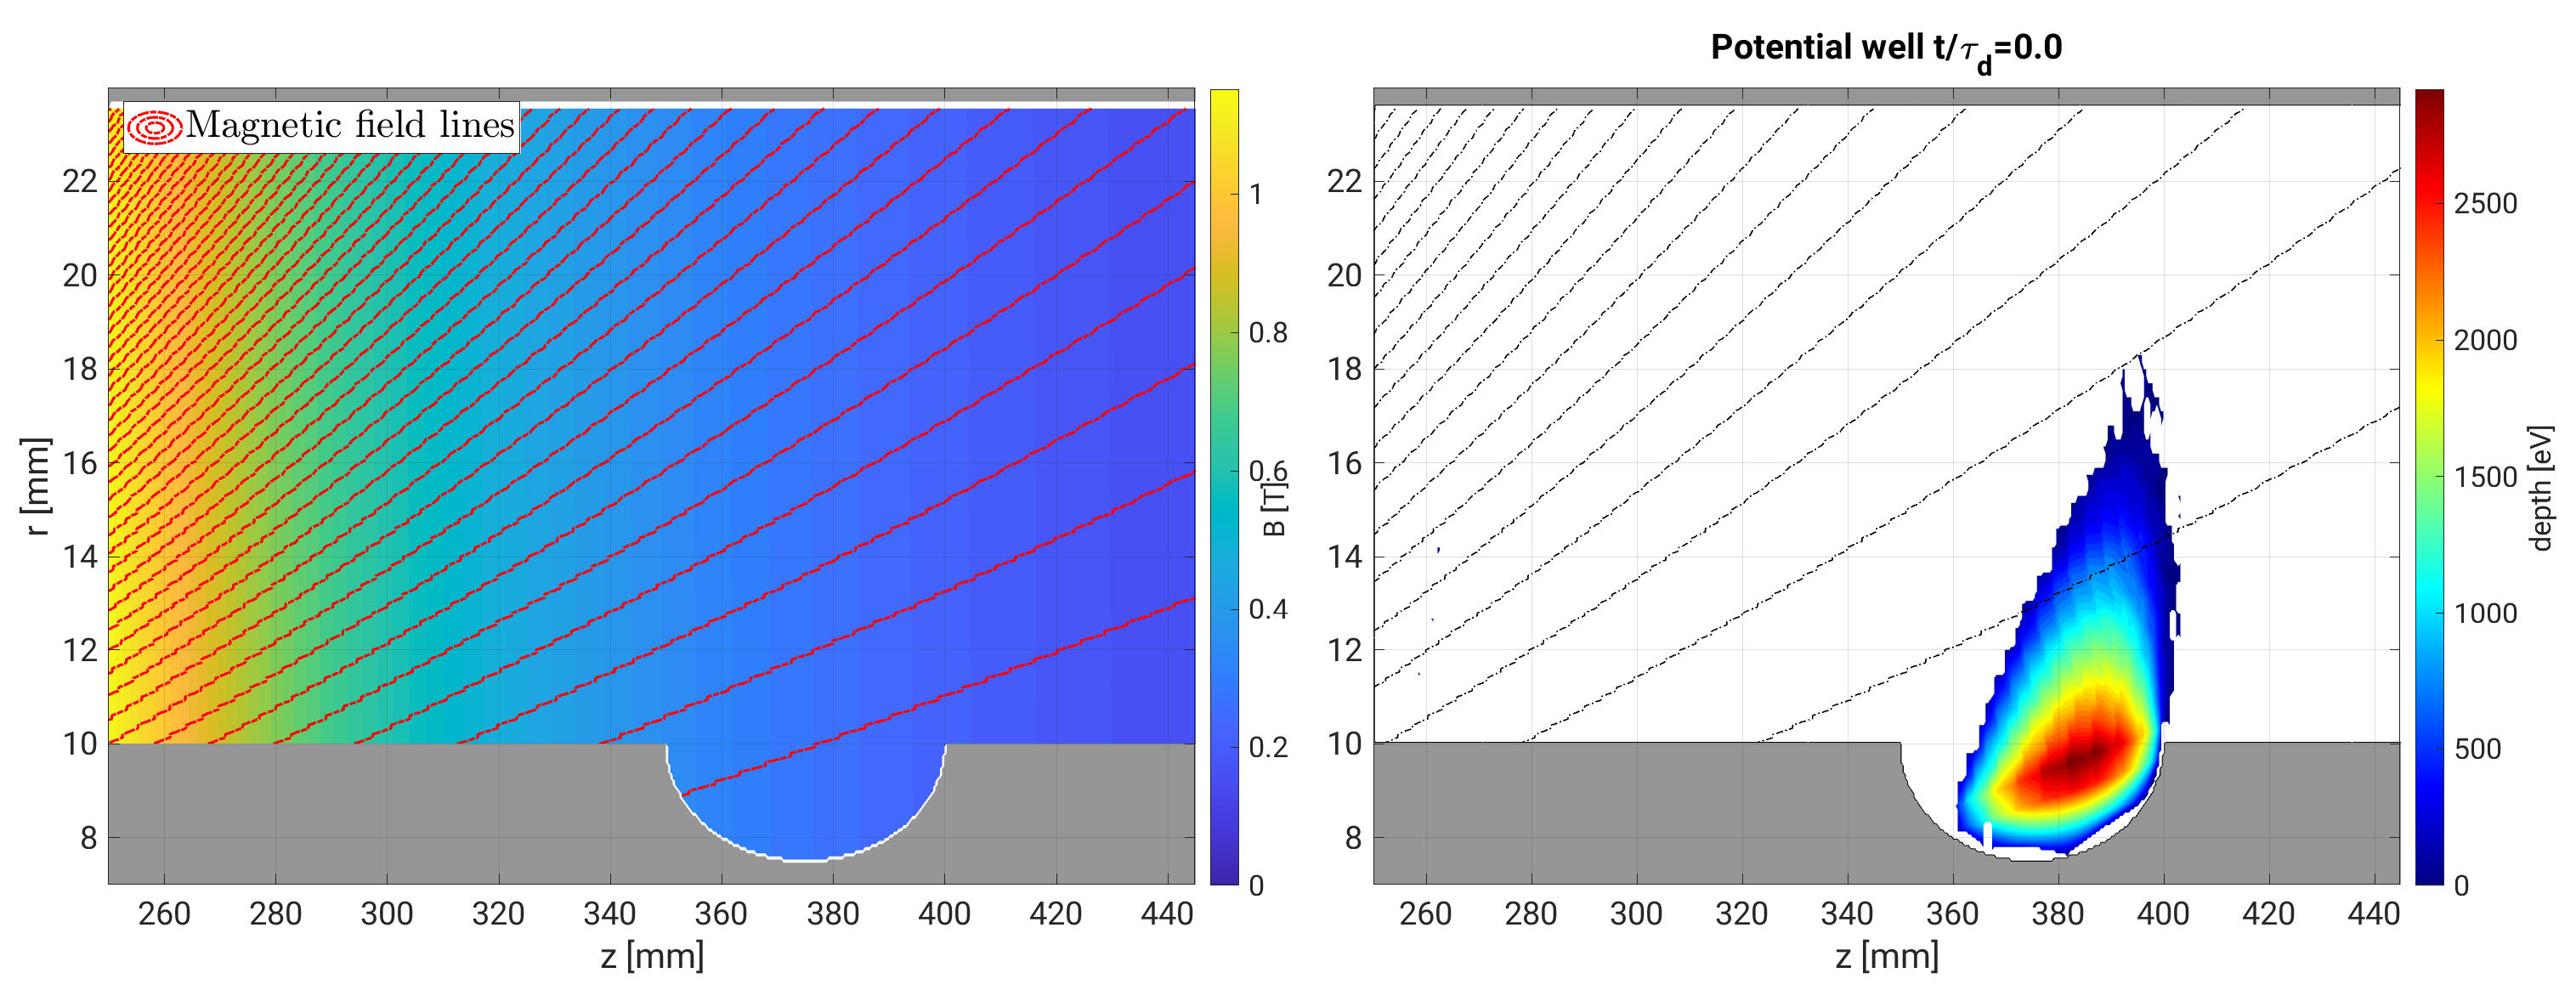
\includegraphics[width = 1 \textwidth]{Extrude_config_both.eps}
	\caption{\label{extrude_config_both} Left: magnetic configuration for the extrude geometry. The high field side is on the left and the magnetic field lines are shown in red. - Right: Vacuum potential well in the same geometry.}
\end{figure}

In order to carry out the same kind of study as for the slanted configuration, several cases have been studied, the main goal being to compare the characteristics of electron clouds formation with and without IIEE, and how the electric currents collected at the boundaries of the domain are affected too. Let us first review the cloud formation times. It has been stated previously how the steady stated is characterised, especially through the total charge evolution. The absolute value of the total electronic charge in the domain is plotted over normalised time, in the left plot of Fig.(\ref{totcharge_iiee_less}). The striking information is that here, contrarily to the case with the outer ellipse, the steady state is reached much faster. Indeed, the plateau is reached with IIEE about twice as fast as without.\\

\begin{figure}[h!]
\centering
	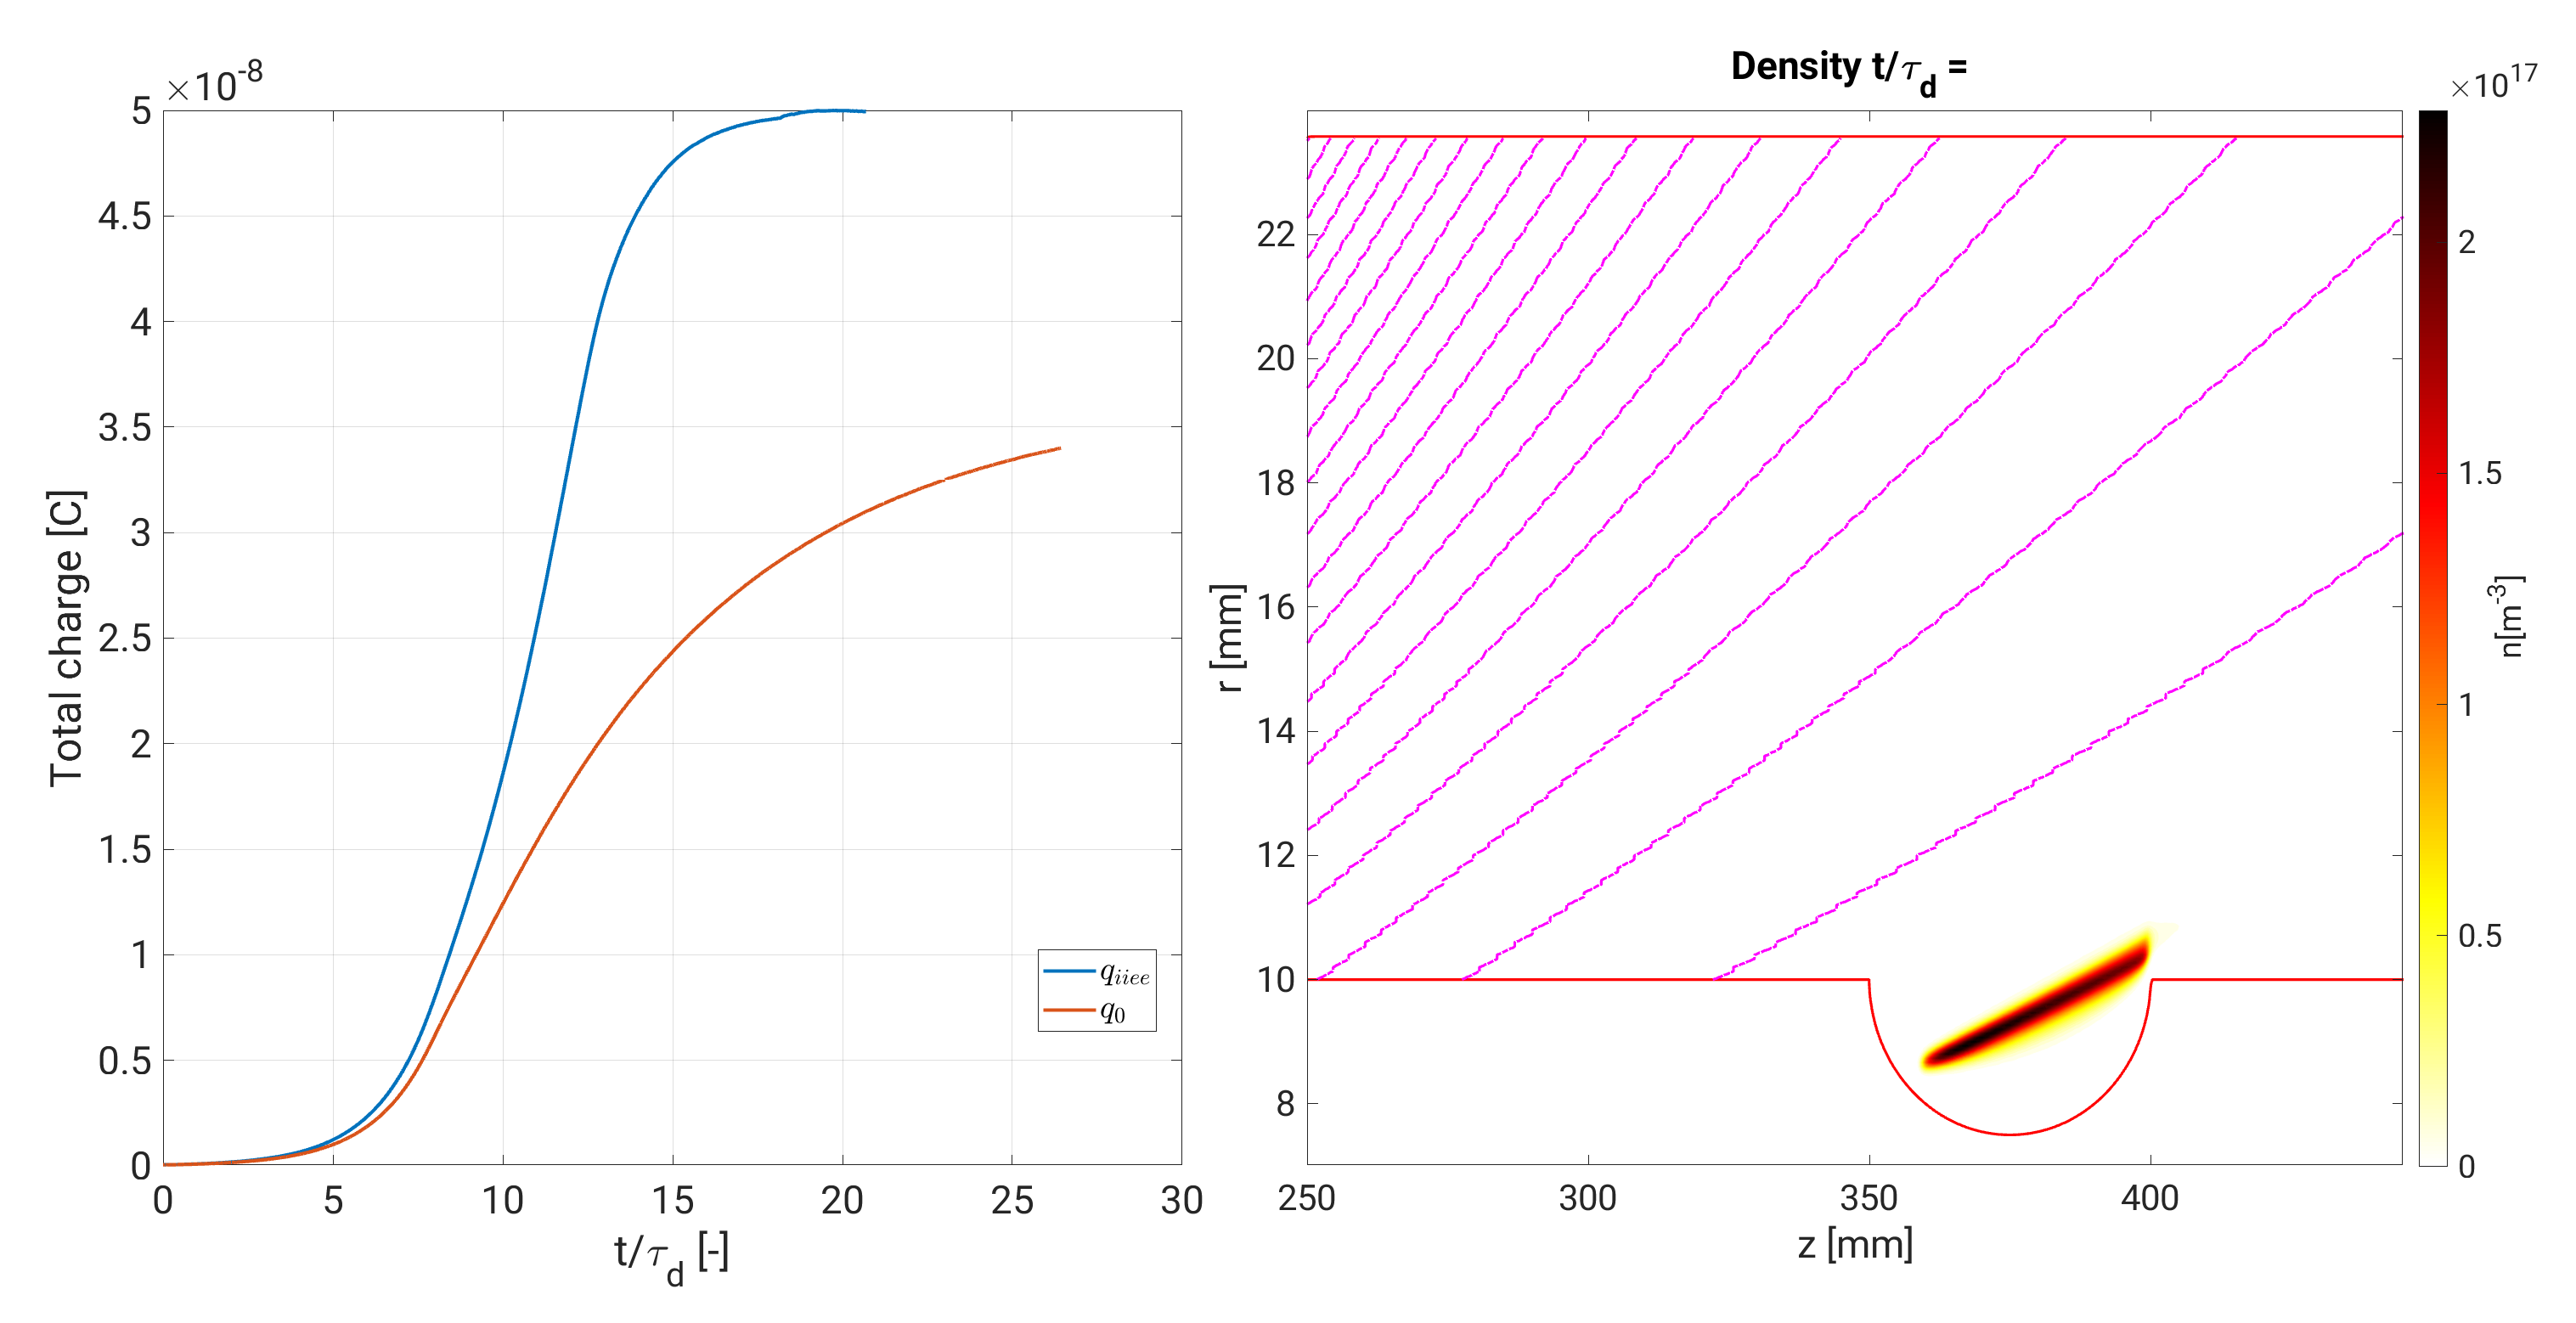
\includegraphics[width = 1 \textwidth]{totcharge_iiee_less.eps}
	\caption{\label{totcharge_iiee_less} Left: total (absolute) charge in the domain over normalised time. - Right: Final state and cloud density in absence of ion induced electron emissions.}
\end{figure}

\noindent The equilibrium state of the cloud without ion induced electrons is shown on the right plot from Fig.(\ref{totcharge_iiee_less}). To be able to compare the latter, the cloud in steady state with IIEE is shown in Fig.(\ref{steady_state_cloud_extrude}). Both the right and left plots are with IIEE, but different initial conditions. This will be discussed below. Coming back to the steady state cloud densities, with and without IIEE, they are of the same order. However, note that the cloud positions are different. The cloud formed in presence of ion induced emissions is located a bit lower inside the ellipse than without. This can be explained by the fact that a lot of electrons being generated at the cathode boundary, in the trapping region, the potential well tends to be filled by the bottom. As the density grows inside the well, the latter becomes progressively narrower and its depth is decreasing as the potential is screen by the charge density (see Fig.(\ref{potential_well_extrude_both}) - Right). Without ion induced emissions (Fig.(\ref{potential_well_extrude_both}) - Right), the well tends to be filling by the top, since the electrons are being generated mostly in the ellipse region, not at the cathode surface. This explains the fact that the potential well remains deep in its bottom part, and hence the upper position of the cloud.\\

\begin{figure}[h!]
\centering
	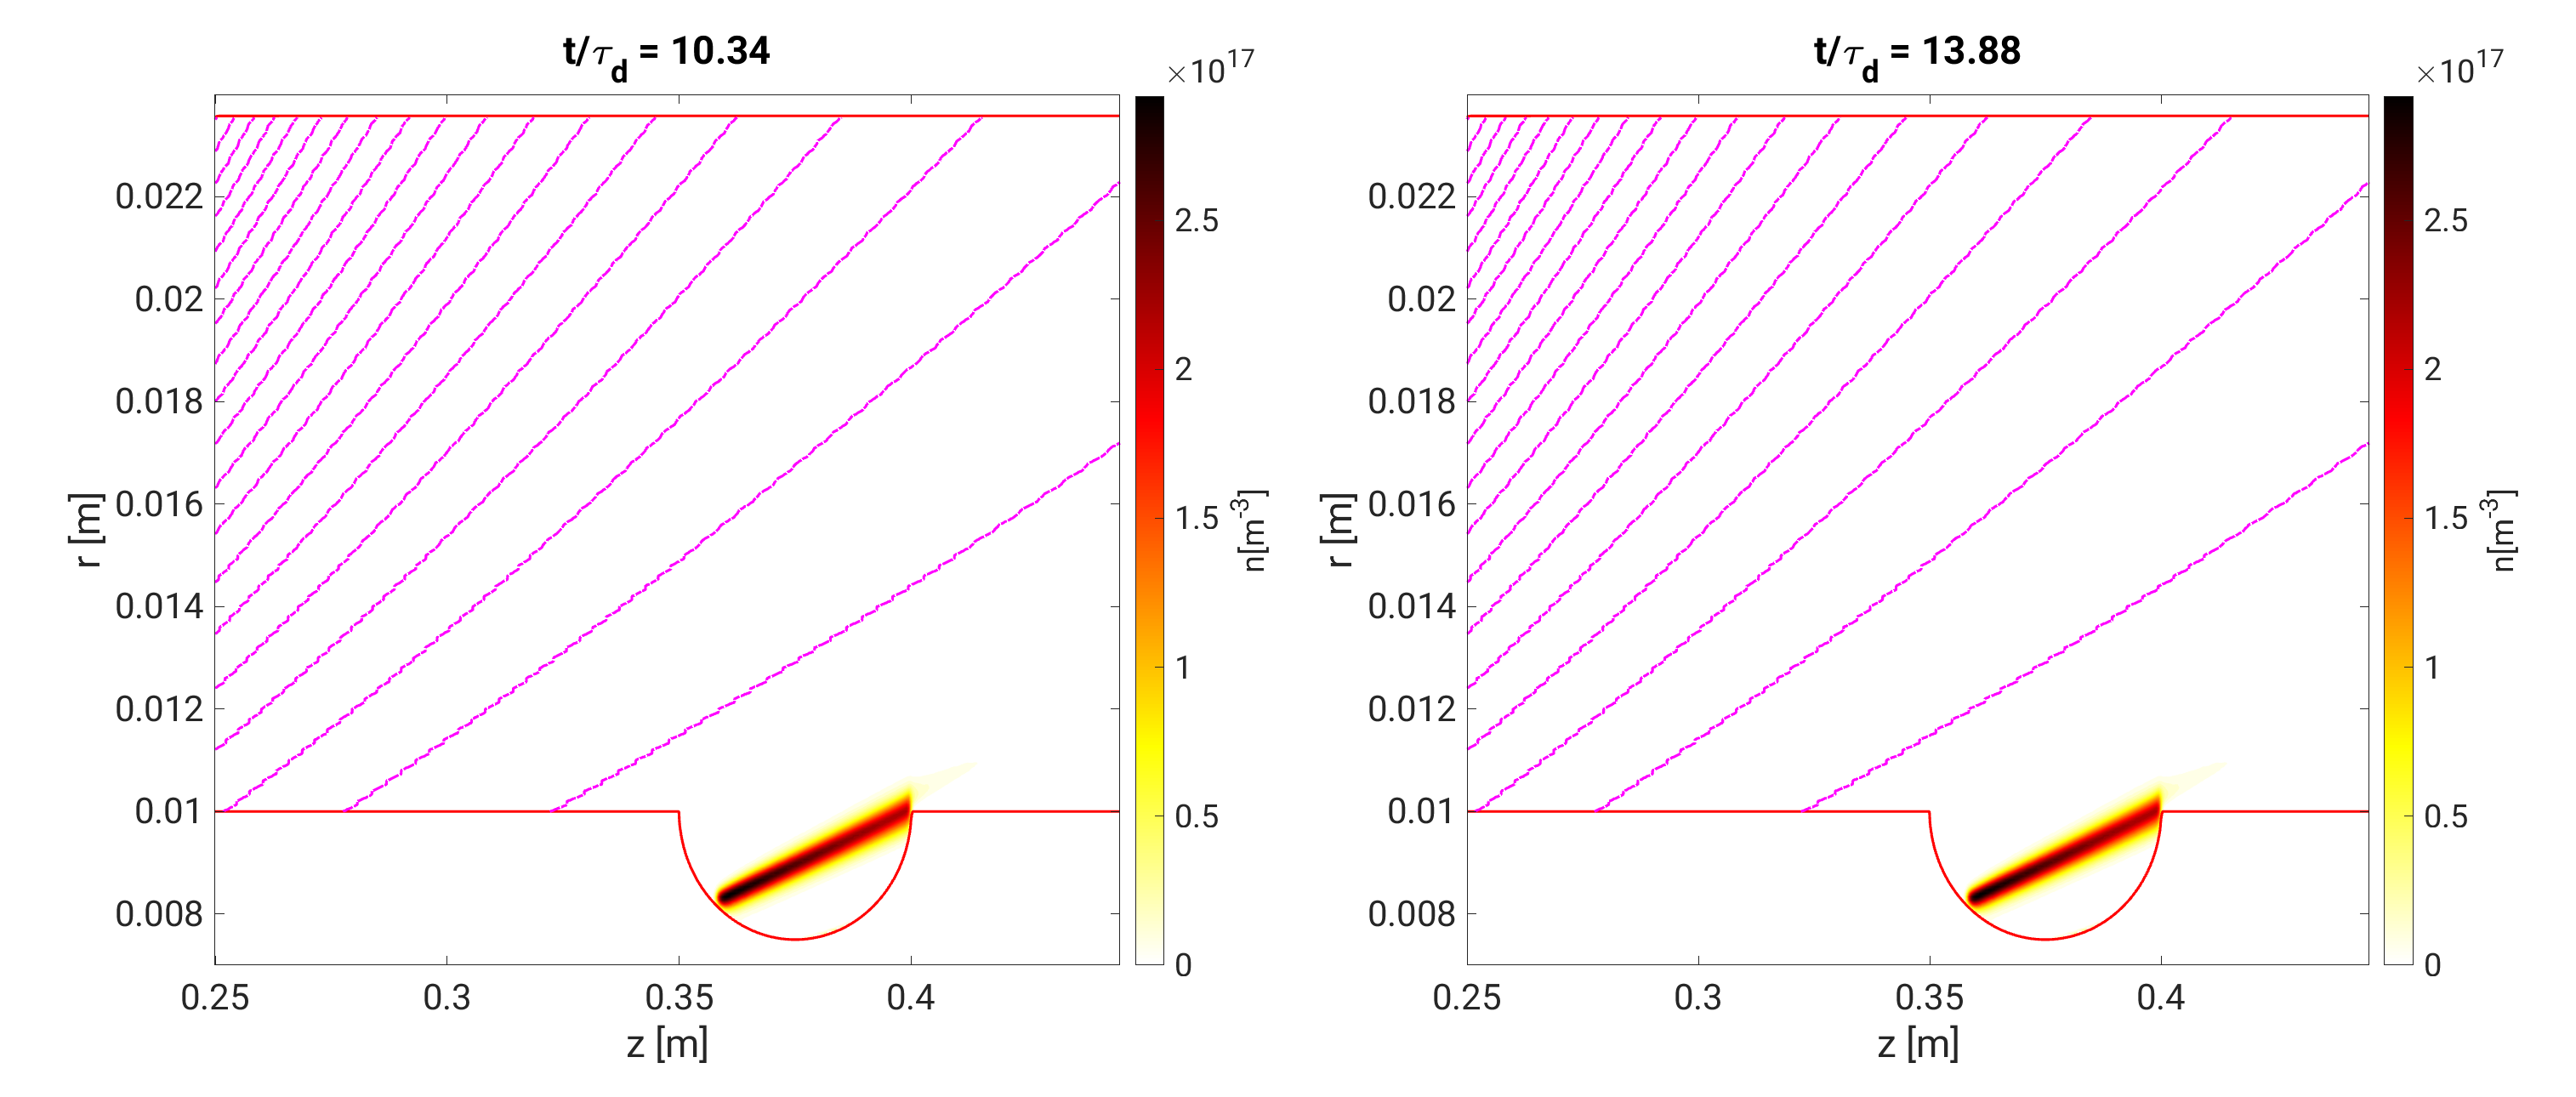
\includegraphics[width = 1 \textwidth]{steady_state_cloud_extrude.eps}
	\caption{\label{steady_state_cloud_extrude} Steady state electron clouds with ion induced electron emissions, corresponding respectively to the left and right initial electron distributions from Fig.(\ref{Config_extrude}).}
\end{figure}

The formation of this particular cloud is the result of a self sustained process arising from IIEE, since according to Fig.(\ref{steady_state_cloud_extrude}) and Fig.(\ref{Config_extrude}), different configurations can lead to this equilibrium. Indeed, the initial electrons and ions do not need to be generated in the region of trapping, inside the ellipse. However, due to the fact that the Larmor radius of the ions is of the order the meter (see Sec.(\ref{fennecs_section})), they travel almost in straight line towards the cathode, so they need to be formed above the ellipse for the induced electrons to be generated in the trapping region. In fact, if the ions were to be formed elsewhere, say in high field region, the electrons that would be induced at the cathode surface would just be lost at the low field side, after being guided along magnetic field lines. Note that the formation time is a variable of the initial electron distribution. Indeed, the more electrons and ions initially present in the ellipse region, the shorter the formation time. The times indicated in Fg.(\ref{steady_state_cloud_extrude}) correspond to the times when configuration reached the same peak density.\\


\begin{figure}[h!]
\centering
	\includegraphics[width = 1 \textwidth]{Config_extrude.eps}
	\caption{\label{Config_extrude} Initial electron distributions leading to the clouds shown in Fig.(\ref{steady_state_cloud_extrude}), taking account for ion induced electron emissions.}
\end{figure}

The last part of this study in the extrude geometry is dedicated to the currents collected at the boundaries of the domain. 

\begin{figure}[h!]
\centering
	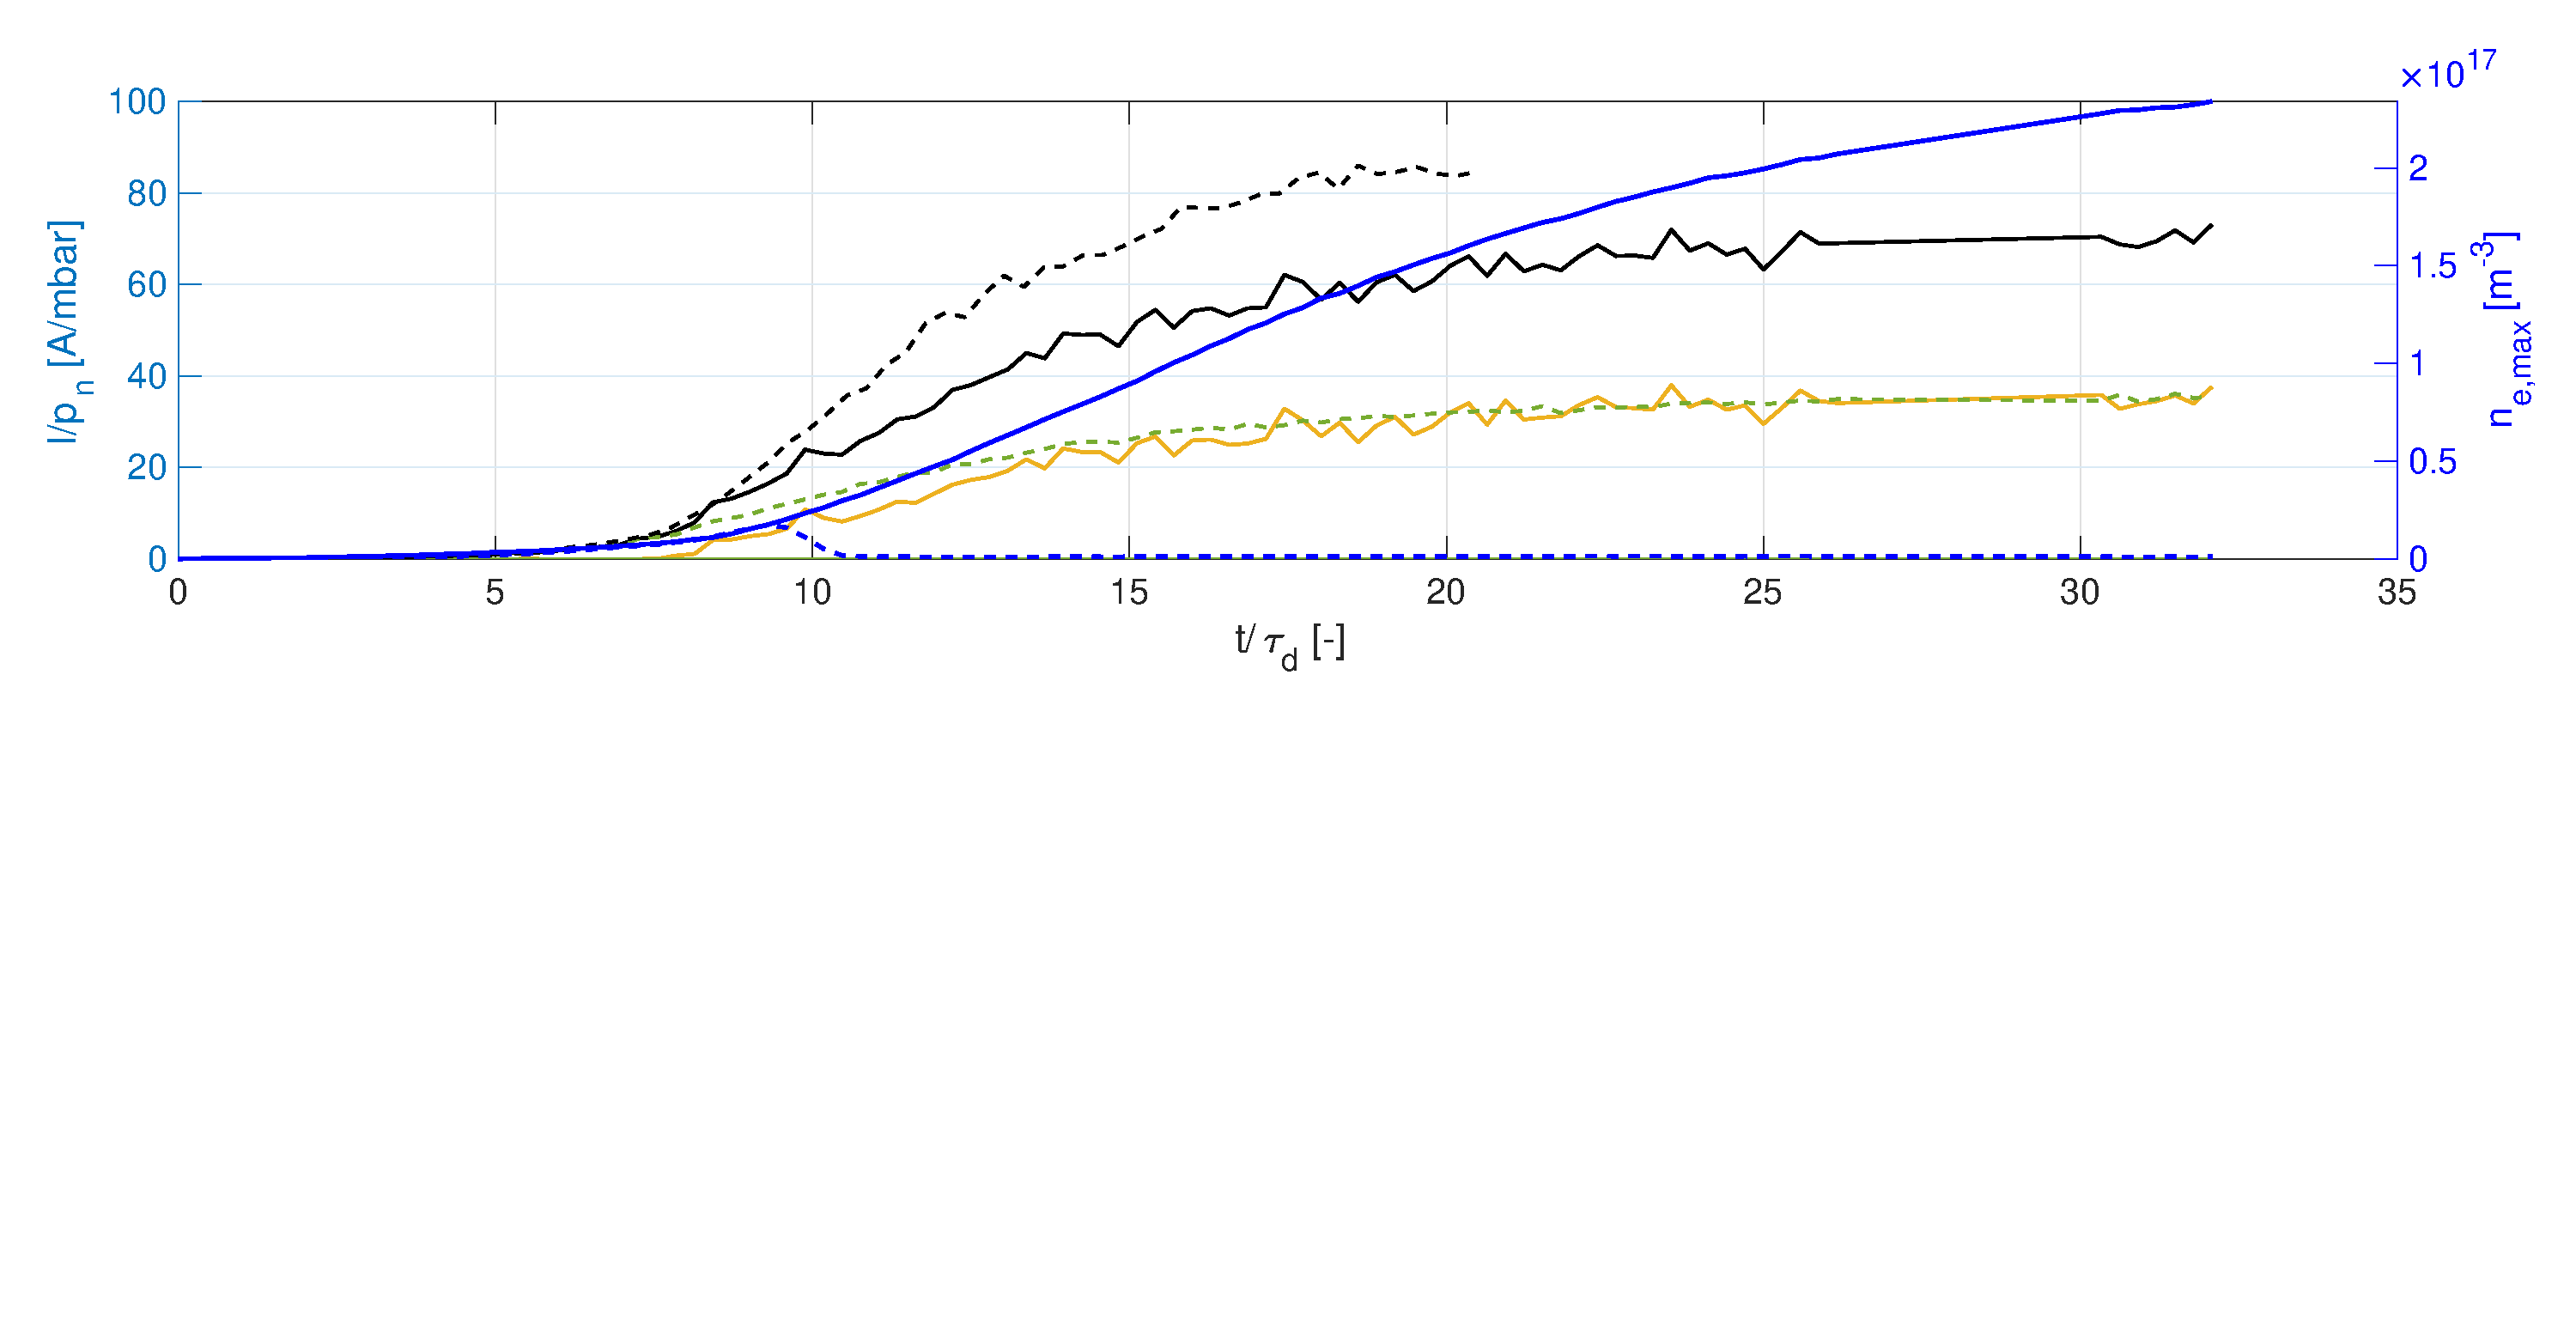
\includegraphics[width = 1 \textwidth]{TotCurr_Extrude_iiee_less.pdf}
	\caption{\label{TotCurr_Extrude_iiee_less} Current collected at all the domain boundaries, without ion induced electron emissions. The color code is the same as the one used for the slanted geometry. The total current from Fig.(\ref{TotCurr_Extrude_iiee}) has been superimposed for the sake of comparison. However the curve is interrupted earlier since the steady state was reached much faster.}
\end{figure}

\begin{figure}[h!]
\centering
	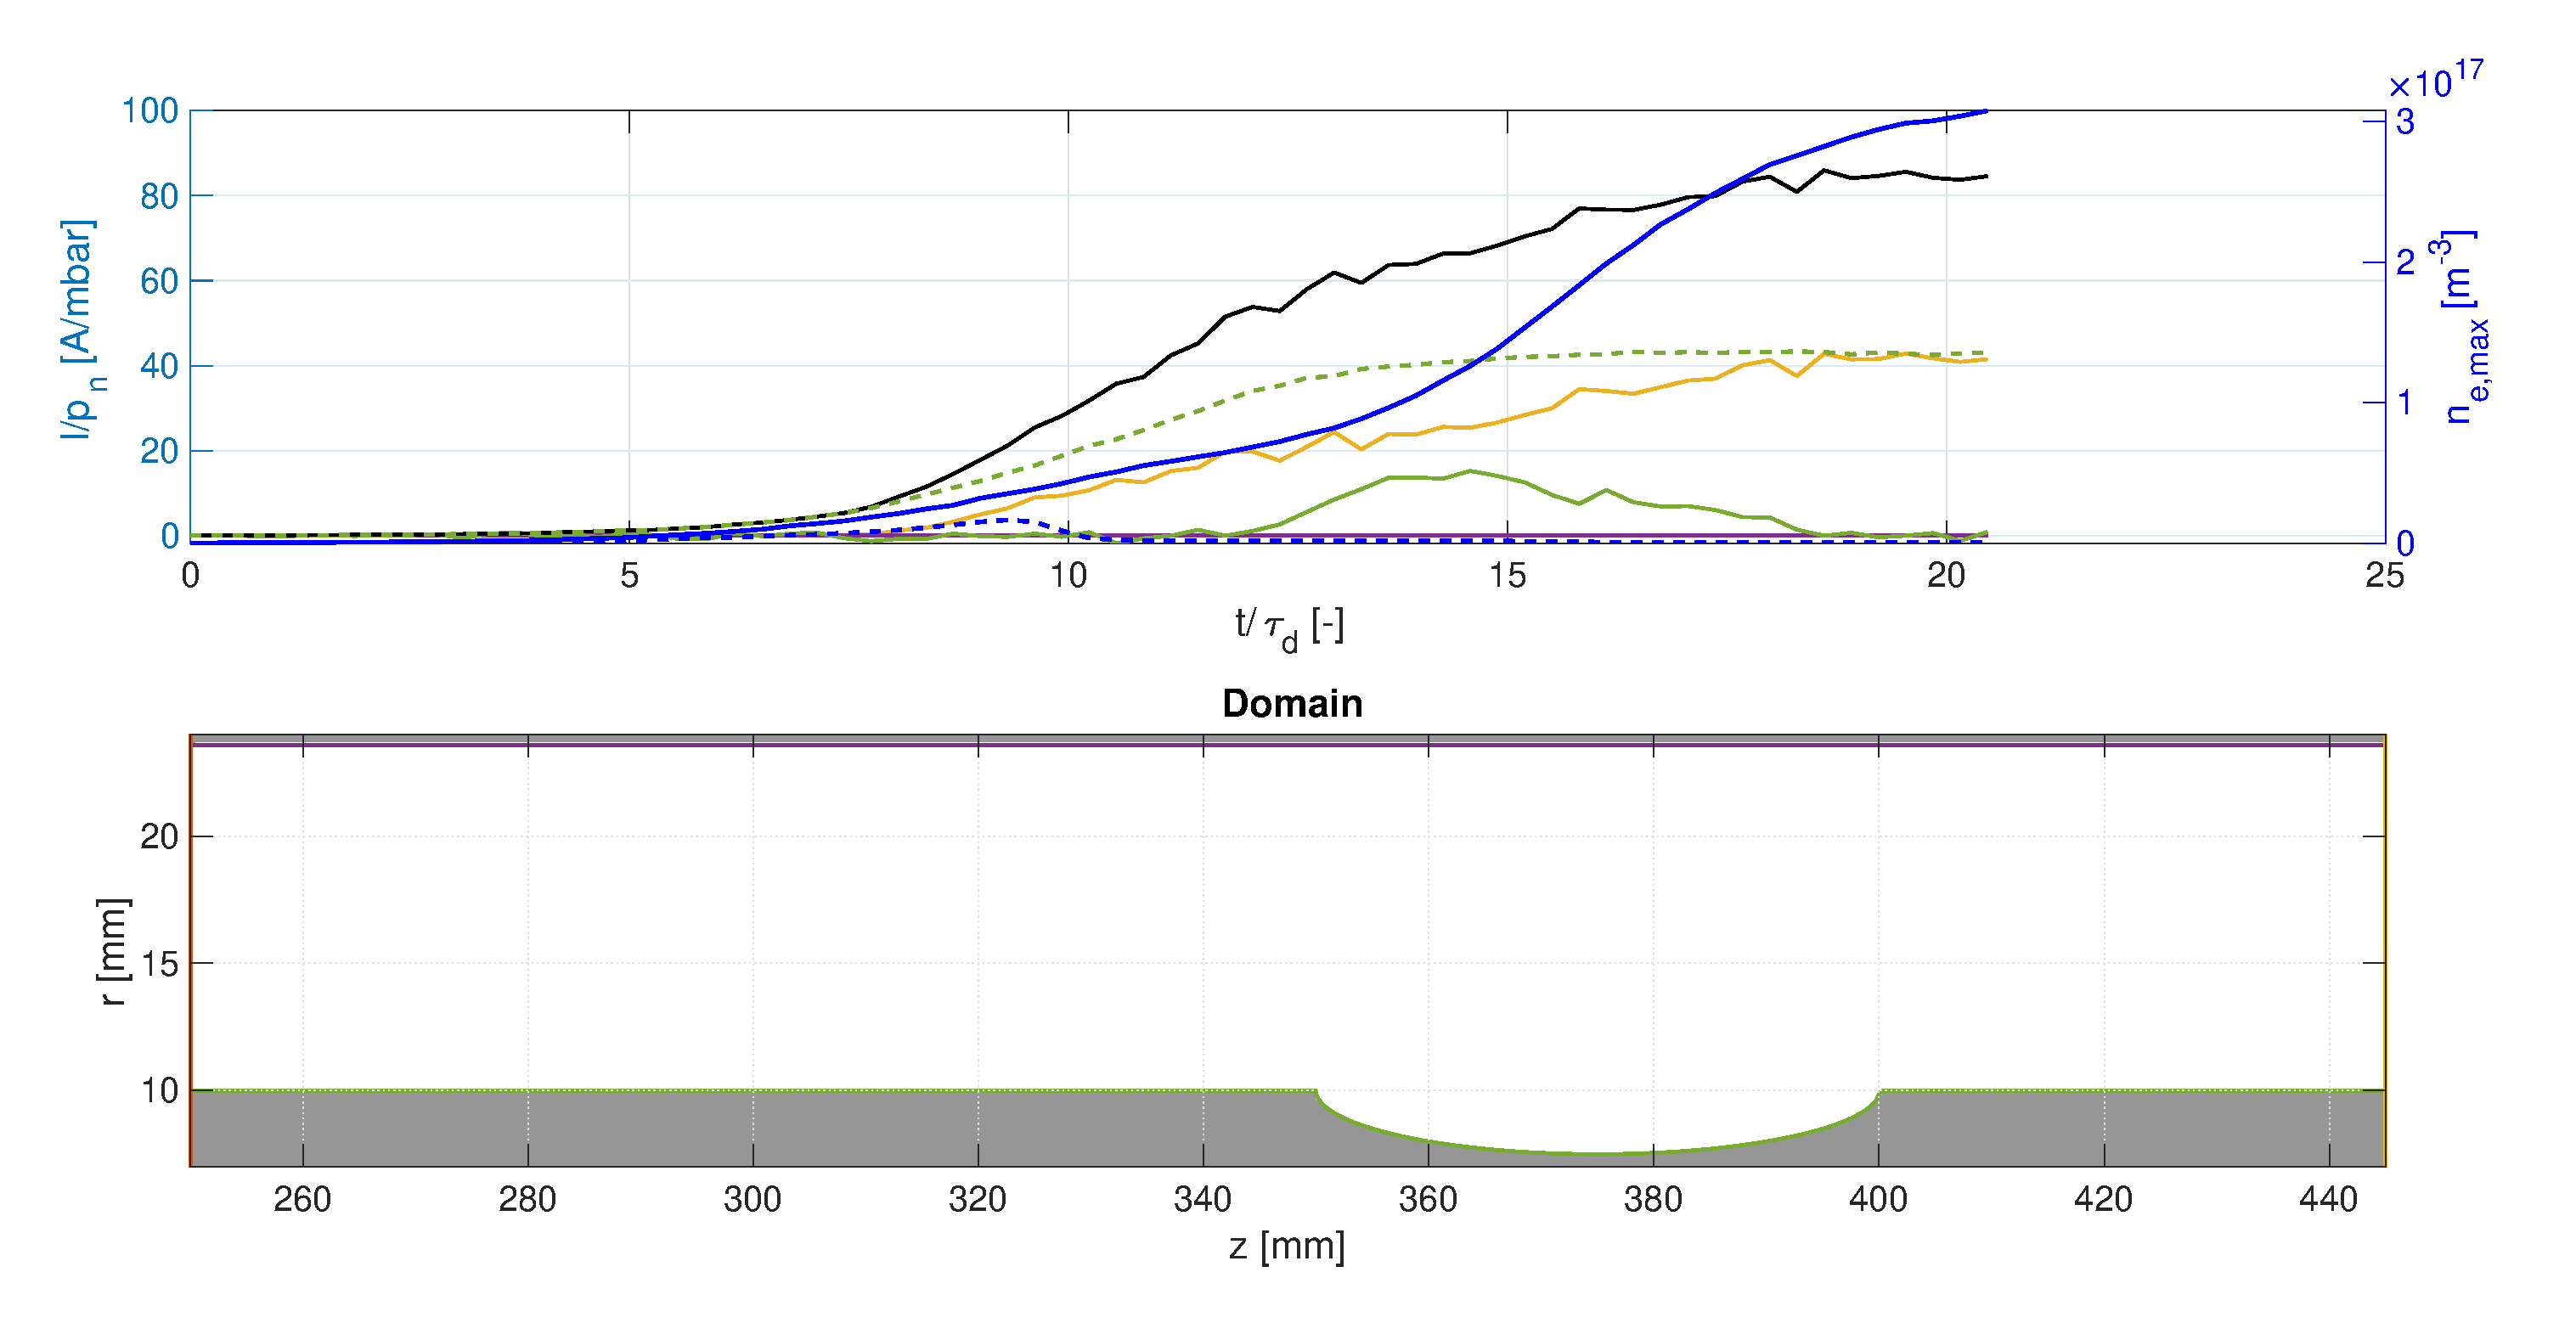
\includegraphics[width = 1 \textwidth]{TotCurr_Extrude_iiee.eps}
	\caption{\label{TotCurr_Extrude_iiee} Current collected at all the domain boundaries, with IIEE. The color of the curves matches the highlighted domain boundaries. The dashed green still represents the ionic current at the cathode.  }
\end{figure}


\begin{figure}[h!]
\centering
	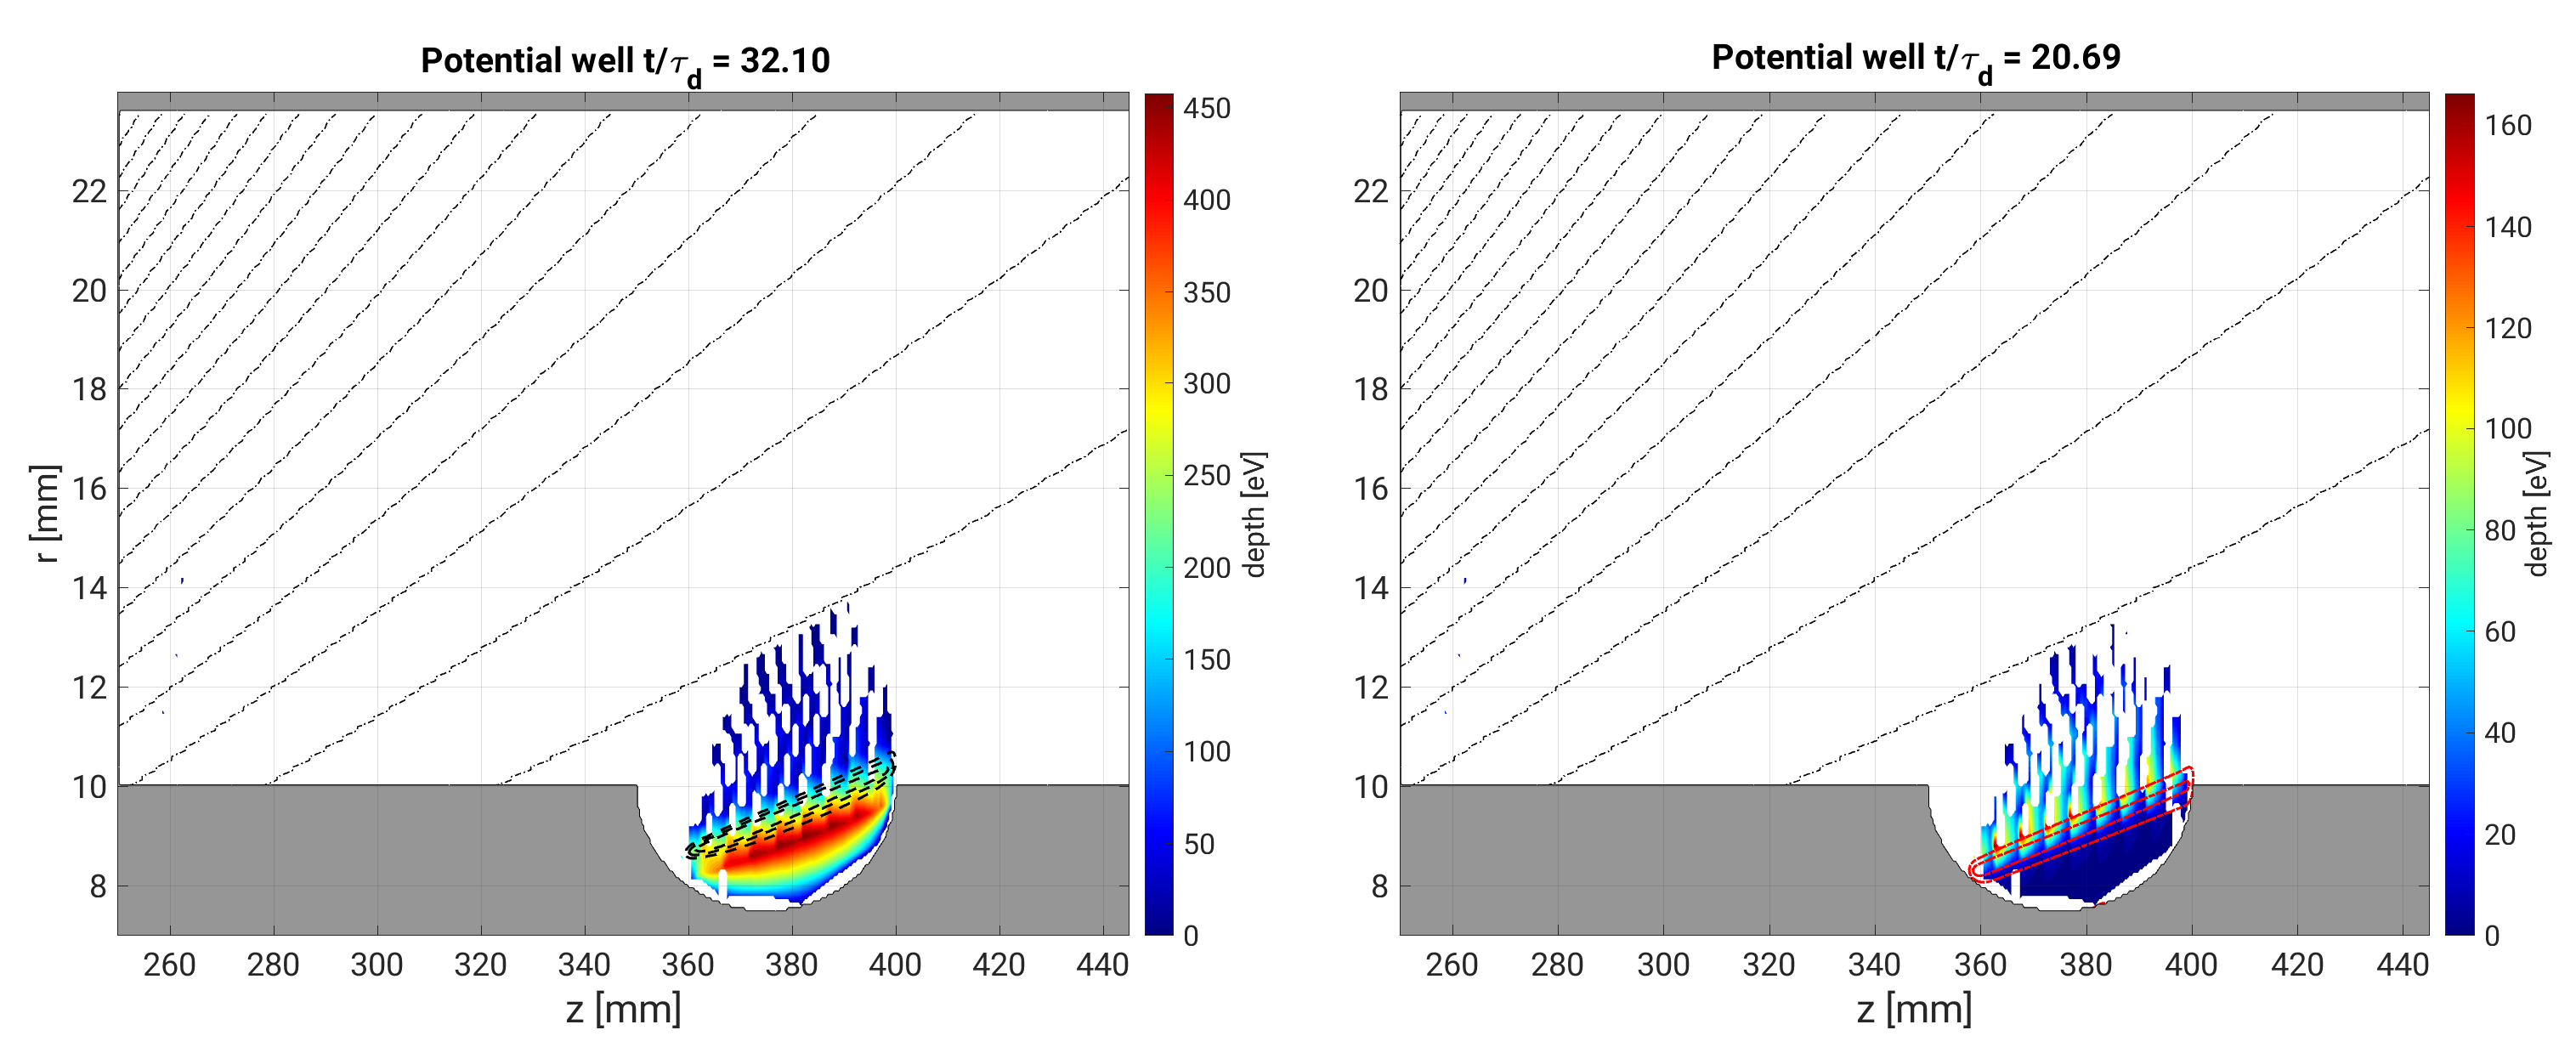
\includegraphics[width = 1 \textwidth]{potential_well_extrude_both.eps}
	\caption{\label{potential_well_extrude_both} Left: Potential well in presence of the cloud, in steady state, without ion induced emissions. Some cloud density contours are given in dashed black. The innermost contour has a greater density than the outermost. Right: Same, but with ion indued emissions. For readability purpose, the density contours are shown in red. The time has been normalised.}
\end{figure}


\newpage
\textbf{ITER gt-170 refurbished MIG}\\

\newpage
\subsection{Further implementation}